\documentclass[11pt]{article}
	
	%%%%%%%%%%%%%%%%%%%%%%%%%%%%%%%%%%%%%%%%%%%%%%%%%%%%%%%%%%%%%%%%%%%%%%
	%\pdfminorversion=4
	% NOTE: To produce blinded version, replace "0" with "1" below.
	\newcommand{\blind}{0}
	
	%%%%%%% IISE Transactions margin specifications %%%%%%%%%%%%%%%%%%%
	% DON'T change margins - should be 1 inch all around.
	\addtolength{\oddsidemargin}{-.5in}%
	\addtolength{\evensidemargin}{-.5in}%
	\addtolength{\textwidth}{1in}%
	\addtolength{\textheight}{1.3in}%
	\addtolength{\topmargin}{-.8in}%
    \makeatletter
    \renewcommand\section{\@startsection {section}{1}{\z@}%
                                       {-3.5ex \@plus -1ex \@minus -.2ex}%
                                       {2.3ex \@plus.2ex}%
                                       {\normalfont\fontfamily{phv}\fontsize{16}{19}\bfseries}}
    \renewcommand\subsection{\@startsection{subsection}{2}{\z@}%
                                         {-3.25ex\@plus -1ex \@minus -.2ex}%
                                         {1.5ex \@plus .2ex}%
                                         {\normalfont\fontfamily{phv}\fontsize{14}{17}\bfseries}}
    \renewcommand\subsubsection{\@startsection{subsubsection}{3}{\z@}%
                                        {-3.25ex\@plus -1ex \@minus -.2ex}%
                                         {1.5ex \@plus .2ex}%
                                         {\normalfont\normalsize\fontfamily{phv}\fontsize{14}{17}\selectfont}}
    \makeatother
    %%%%%%%%%%%%%%%%%%%%%%%%%%%%%%%%%%%%%%%%%%%%%%%%%%%%%%%%%%%%%%%%%%%%%%%%%
	
	%%%%% IISE Transactions package list %%%%%%%%%%%%%%%%%%%%%%%%%%%%%%%%%%%%%%
	\usepackage{amsmath}
	\usepackage{graphicx}
	\usepackage{enumerate}
	\usepackage{natbib} %comment out if you do not have the package
	\usepackage{url} % not crucial - just used below for the URL
    \usepackage{xcolor}
    \usepackage{enumitem}
    \usepackage{amssymb}
    \usepackage{algorithm}
%    \floatstyle{plaintop} % 设置标题在顶部，且没有默认的粗横线
%    \restylefloat{algorithm}
    \usepackage{algpseudocode}
    \usepackage{bm}
    \usepackage{setspace}
    \usepackage{float} % 需要这个包来控制样式
    \usepackage{graphicx}
    \usepackage{subcaption}
    \usepackage{booktabs} % 用于专业表格线条 (\toprule, \midrule, \bottomrule)
    \usepackage{multirow} % 用于合并单元格 (\multirow)

	%%%%%%%%%%%%%%%%%%%%%%%%%%%%%%%%%%%%%%%%%%%%%%%%%%%%%%%%%%%%%%%%%%%%%%%
	
	%%%%% Author package list and commands %%%%%%%%%%%%%%%%%%%%%%%%%%%%%%%%%%%%%%%%%%%%%
	%%%%% Here are some examples %%%%%%%%%%%%%%
	%	\usepackage{amsfonts, amsthm, latexsym, amssymb}
	%	\usepackage{lineno}
	%	\newcommand{\mb}{\mathbf}
	%%%%%%%%%%%%%%%%%%%%%%%%%%%%%%%%%%%%%%%%%%%%%%%%%%%%%%%%%%%%%%%%%%%%%%%%%%%%%%
	
	\begin{document}
		
			%%%%%%%%%%%%%%%%%%%%%%%%%%%%%%%%%%%%%%%%%%%%%%%%%%%%%%%%%%%%%%%%%%%%%%%%%%%%%%
		\def\spacingset#1{\renewcommand{\baselinestretch}%
			{#1}\small\normalsize} \spacingset{1}
		%%%%%%%%%%%%%%%%%%%%%%%%%%%%%%%%%%%%%%%%%%%%%%%%%%%%%%%%%%%%%%%%%%%%%%%%%%%%%%
		
	\if0\blind
	{
		\title{Dual-Attention Deep Gaussian Processes for Multi-Objective Robust Parameter Design}
%		\author{Zebiao Feng $^a$, Xu Yang $^a$, Xiaojian Zhou $^a$ and Jianjun Wang $^b$\thanks{Corresponding author: Jianjun Wang (email: \texttt{jjwang@njust.edu.cn})} \\
%			$^a$ \parbox{1\textwidth}{School of Management, Nanjing University of Posts and Telecommunications, Nanjing 210003, China} \\
%			$^b$ \parbox{1\textwidth}{Department of Management Science and Engineering, Nanjing University of Science and Technology, Nanjing 210094, China}}
%		\date{}
		\maketitle
	} \fi
	
		
		\if1\blind
		{

            \title{Dual-Attention Deep Gaussian Processes for Multi-Objective Robust Parameter Design}
			\author{Zebiao Feng $^a$, Xu Yang $^a$, Xioajian Zhou $^a$ and Jianjun Wang $^b$\thanks{Corresponding author: Jianjun Wang (email: \texttt{jjwang@njust.edu.cn})} \\
				$^a$ \parbox{1\textwidth}{School of Management, Nanjing University of Posts and Telecommunications, Nanjing 210003, China} \\
				$^b$ \parbox{1\textwidth}{Department of Management Science and Engineering, Nanjing University of Science and Technology, Nanjing 210094, China}}
			
\bigskip
			\bigskip
			\bigskip
			\begin{center}
				{\LARGE\bf \emph{IISE Transactions} \LaTeX \ Template}
			\end{center}
			\medskip
		} \fi
		\bigskip
		
	\begin{abstract}
Robust parameter design (RPD) for modern complex engineering systems is frequently challenged by small sample sizes, non-stationary response surfaces, and strongly conflicting objectives. Existing Gaussian process (GP) surrogate models, constrained by global stationarity assumptions and mean-oriented loss functions, often suffer from underfitting in the region of interest (ROI) critical for optimization. To overcome these limitations, this paper proposes a novel modeling framework named dual-attention deep Gaussian process (DA-DGP). A hierarchical attention mechanism is constructed: at the data level, a sample-level attention is designed to assign higher learning weights to samples within the ROI, achieving refined local modeling of potential optimal regions; at the task level, a meta-learning-based dynamic weight adjustment strategy is introduced to effectively mitigate gradient conflicts among heterogeneous objectives. By deriving a rigorous weighted variational evidence lower bound (ELBO), the framework realizes end-to-end joint optimization of model parameters and attention weights. Experiments on benchmarks and a 5G/6G OFDM design confirm that DA-DGP consistently outperforms all baselines, reducing the RMSE by 9.9\%–19.1\% in numerical tasks and the error vector magnitude by 2.7\%–19.2\% in the engineering case, respectively.
	\end{abstract}
			
	\noindent%
	{\it Keywords:} Robust parameter design; deep Gaussian processes; dual-attention mechanism; multi-objective optimization; computer experiments

	%\newpage
	\spacingset{1.5} % DON'T change the spacing!


\section{Introduction} \label{s:intro}

Robust parameter design (RPD) serves as a cornerstone of modern industrial quality engineering. It aims to optimize controllable design factors to minimize the deviation of system output responses from target values while significantly reducing performance variations induced by uncontrollable noise factors \citep{Taguchi1986, Joseph2006, Montgomery2017, Hamada2021}. In advanced engineering applications such as aerospace, radar electronic countermeasures, and 5G/6G communication systems, product quality responses often exhibit highly nonlinear and multimodal characteristics \citep{Wang2020, Liu2025, Gnanasambandam2025, SongJ2025}. Taking orthogonal frequency division multiplexing (OFDM) as an example—a core physical layer technology in communication systems—despite its superior resistance to multipath fading, its practical deployment faces challenging multi-objective conflict problems. Specifically, increasing transmission power can improve the signal-to-noise ratio (SNR), thereby enhancing throughput and reducing the bit error rate (BER); however, this inevitably leads to a deterioration in the peak-to-average power ratio (PAPR) and a surge in energy consumption. This complex coupling relationship is governed by a series of intricate signal processing procedures, such as IFFT transformation, cyclic prefix insertion, and multipath channel convolution, resulting in high nonlinearity and typical “black-box” attributes. However, high-fidelity physical layer link simulations (involving steps such as random pilots and least squares channel estimation) are computationally expensive. A single link evaluation often requires millions of floating-point operations to resolve complex signal convolutions \citep{Song2025}. Furthermore, large-scale field testing is constrained by electromagnetic environments and prohibitive costs, leading to an extreme scarcity of high-quality samples available for modeling \citep{Ming2022, Sauer2022, Ghandwani2025}. Therefore, employing surrogate modeling to construct low-cost mathematical approximations of the real physical layer has become a key paradigm for addressing such optimization problems characterized by small sample sizes and multiple conflicting objectives \citep{Luo2022, LiY2025}.

Among various surrogate models, Gaussian processes (GP) have become the preferred tool for addressing such small-sample regression problems due to their nonparametric flexibility and capability for uncertainty quantification (UQ) \citep{Williams2006, Deng2017, Joseph2019}. Unlike traditional parametric models, GPs utilize kernel functions to capture correlations among input variables, enabling the simultaneous prediction of response means and variances—a characteristic that inherently aligns with the ``mean-variance'' joint modeling requirement in robust parameter design \citep{Gramacy2020, Wang2025}. However, standard GPs typically rely on a single global stationary kernel, assuming uniform smoothness across the input space. This assumption limits their ability to capture multi-scale, abrupt, or non-stationary response surfaces \citep{Ko2022, Sauer2023, Tao2025}. Taking the OFDM communication system focused on in this paper as an example, influenced by the nonlinear coupling of carrier frequency offset drift and multipath effects, its BER response surface often exhibits drastic ``cliff-like'' abrupt changes, while the PAPR presents complex non-Gaussian distributions. Due to a lack of hierarchical feature extraction capabilities, single-layer (shallow) GPs struggle to accurately characterize such complex non-stationary interactions in high-dimensional spaces \citep{Zhai2022, Lin2024, WangX2025}. To overcome this limitation, deep Gaussian processes (DGP) have emerged \citep{Damianou2013}. By mapping the input space to a latent feature space through a multi-layer cascaded GP structure, DGPs possess strong capabilities for modeling non-stationary functions, demonstrating significant advantages in handling complex physical field simulations \citep{Muller2017, Ding2024}. 

Nevertheless, existing DGP modeling frameworks still possess a core deficiency when dealing with robust parameter optimization tasks: their standard variational inference processes typically aim to maximize the global evidence lower bound (ELBO), essentially seeking to minimize the average fitting error across the entire input space. This ``averaging'' global loss function causes the model to tend towards smoothing global trends, often resulting in underfitting in the region of interest (ROI) that is critical for robust optimization \citep{Zhang2022}. Due to the lack of a mechanism to ``focus'' model capacity on key subspaces, limited computational resources are dispersed over low-performance regions irrelevant to optimization, severely limiting the potential for efficient robust optimization under extremely small sample conditions.

In light of the limitations inherent in traditional models that treat data indiscriminately, the attention mechanism—as a technique capable of dynamically filtering key information—has achieved significant success in deep learning and industrial intelligence in recent years \citep{Cho2024, Guo2025}. For instance, in fault diagnosis and remaining useful life (RUL) prediction tasks, models can effectively suppress redundant noise and enhance prediction accuracy by adaptively assigning weights to different feature channels or time steps \citep{Fan2025, Ma2025}. Inspired by these advancements, the academic community has recently begun attempting to introduce attention mechanisms into the Gaussian process domain: \cite{Schmidt2024} proposed a probabilistic attention method to improve deep multiple instance learning, while \cite{Nakamura2021} applied self-attention layers to sequence-to-sequence speech generation tasks. 
However, existing integration methods are mostly confined to single-layer attention structures or specific classification and sequence tasks, and have not yet systematically incorporated multi-level attention mechanisms into the hierarchical variational inference framework of DGPs \citep{Booth2025}.  Although recent studies have explored transfer learning strategies \citep{Yao2026} and multi-task structural learning \citep{Yang2025} to enhance modeling efficiency,  particularly in the field of RPD, how to leverage attention weights to simultaneously address the dual challenges of ``sample-level focusing on small samples (Sample Selection)'' and ``task-level trade-offs for multi-objective conflicts (Task Balancing)'' remains systematically unexplored.

Driven by these needs, this paper proposes a novel framework named Dual-attention deep Gaussian process (DA-DGP). Unlike traditional multi-task Gaussian processes that rely on explicit task covariance matrices (e.g., the linear model of coregionalization, LMC), the proposed model utilizes deep structures to implicitly capture complex dependencies among outputs. This framework is specifically tailored for RPD problems characterized by small sample sizes, high-dimensional nonlinearities, and strongly conflicting objectives. The core philosophy is to synergize two attention mechanisms with varying granularities to intelligently guide and allocate limited modeling resources. The main contributions of this paper are summarized as follows:

\begin{enumerate}[label=(\arabic*), wide, labelwidth=!, labelindent=0pt]
	\item \textbf{Sample-level Attention:} To address the local optimization characteristics of RPD, a quality loss function is integrated into the kernel computation. This mechanism guides the model to automatically focus on the target ROI under extremely small sample conditions, effectively improving prediction accuracy in critical subspaces.
	
	\item \textbf{Task-level Attention:} To address the strong conflicts among multiple objectives, a bilevel optimization strategy based on meta-learning is designed. This mechanism adaptively learns the optimal weights for conflicting tasks based on validation set performance, overcoming the limitations of traditional static weighting methods.
	
	\item \textbf{Weighted Variational Inference:} A rigorous weighted variational ELBO is derived, seamlessly integrating the aforementioned dual-attention mechanisms into the end-to-end training of the DGP. This realizes the collaborative optimization of model parameters and attention weights.
	
	\item \textbf{Engineering Validation and Evaluation:} Through standard numerical benchmark functions and a high-dimensional 5G/6G OFDM communication link optimization case, the advantages of the proposed method in handling non-stationary responses, multi-objective conflicts, and small sample data are systematically validated.
\end{enumerate}

The remainder of this paper is organized as follows: Section 2 briefly reviews the theoretical foundations of GPs and DGPs, elucidating the applicability of multi-output DGPs in handling high-dimensional non-stationary responses. Section 3 details the proposed DA-DGP framework, focusing on the construction of the sample-level attention for precisely locating the ROI and the task-level attention mechanism for balancing multi-objective conflicts; furthermore, the weighted ELBO and the multi-objective robust optimization model are derived. Section 4 validates the effectiveness and superiority of the proposed method in small-sample computer experiments through numerical benchmark tests and an engineering case study of a 5G/6G OFDM communication system. Finally, Section 5 concludes the paper and outlines future research directions.

\section{Theoretical Backgrounds} \label{sec:background}

Let $\mathbf{x} \in \mathbb{R}^d$ denote the input design factors and $y \in \mathbb{R}$ be the system response. We aim to construct a surrogate model based on a dataset $\mathcal{D}=\{\mathbf{X}, \mathbf{y}\}$ containing $N$ observations, assuming a noisy relationship $y = f(\mathbf{x}) + \epsilon$ with Gaussian noise $\epsilon \sim \mathcal{N}(0, \sigma_n^2)$.

\subsection{Standard Gaussian Processes} \label{subsec:gp}

A Gaussian Process (GP) places a prior distribution over the latent function $f$, assuming that any finite collection of function values has a joint Gaussian distribution. Formally, the GP prior is specified by a mean function $m(\mathbf{x})$ (assumed zero for simplicity) and a covariance function $k(\mathbf{x}, \mathbf{x}')$:
\begin{equation}
	f(\mathbf{x}) \sim \mathcal{GP}(0, k(\mathbf{x}, \mathbf{x}')).
\end{equation}
To capture the non-linear correlations with different sensitivities across input dimensions, we employ the anisotropic Squared Exponential (SE) kernel with Automatic Relevance Determination (ARD):
\begin{equation}
	k(\mathbf{x}, \mathbf{x}') = \sigma_f^2 \exp \left( - \frac{1}{2} (\mathbf{x} - \mathbf{x}')^T \mathbf{L}^{-1} (\mathbf{x} - \mathbf{x}') \right) + \sigma_n^2 \delta_{ij},
\end{equation}
where $\sigma_f^2$ is the signal variance, $\mathbf{L} = \text{diag}(l_1^2, \ldots, l_d^2)$ contains the characteristic length-scales for each dimension, and $\delta_{ij}$ is the Kronecker delta function.

Conditioned on the dataset $\mathcal{D}$, the posterior predictive distribution at a new test point $\mathbf{x}_*$ follows a Gaussian distribution $p(f_* | \mathbf{X}, \mathbf{y}, \mathbf{x}_*) \sim \mathcal{N}(\mu_*(\mathbf{x}_*), \sigma_*^2(\mathbf{x}_*))$, with moments given by:
\begin{equation}
	\begin{aligned}
		\mu_*(\mathbf{x}_*) &= \mathbf{k}_{*N} (\mathbf{K}_{NN} + \sigma_n^2 \mathbf{I})^{-1} \mathbf{y}, \\
		\sigma_*^2(\mathbf{x}_*) &= k(\mathbf{x}_*, \mathbf{x}_*) - \mathbf{k}_{*N} (\mathbf{K}_{NN} + \sigma_n^2 \mathbf{I})^{-1} \mathbf{k}_{N*} + \sigma_n^2,
	\end{aligned}
\end{equation}
where $\mathbf{K}_{NN} = k(\mathbf{X}, \mathbf{X})$ is the covariance matrix of training data and $\mathbf{k}_{*N} = k(\mathbf{x}_*, \mathbf{X})$. The computational complexity is dominated by the inversion of $(\mathbf{K}_{NN} + \sigma_n^2 \mathbf{I})$, scaling as $\mathcal{O}(N^3)$.



\subsection{Sparse Variational Approximation} \label{s:sec2.2}

To address the cubic computational bottleneck, sparse approximation techniques utilize a set of $M$ inducing points $\mathbf{Z} = [\mathbf{z}_1, \ldots, \mathbf{z}_M]^T$ with $M \ll N$, and corresponding inducing variables $\mathbf{u} = f(\mathbf{Z})$. Following the variational inference framework \citep{Titsias2009}, the intractable true posterior is approximated by a variational distribution $q(\mathbf{u}) = \mathcal{N}(\mathbf{m}, \mathbf{S})$. 

By assuming conditional independence between training points given $\mathbf{u}$, the joint variational posterior factorizes as $q(\mathbf{f}, \mathbf{u}) = p(\mathbf{f}|\mathbf{u})q(\mathbf{u})$. The model parameters and variational parameters are jointly optimized by maximizing the Evidence Lower Bound (ELBO):
\begin{equation}
	\mathcal{L}_{\text{SGP}} = \sum_{i=1}^{N} \mathbb{E}_{q(f_i)} [\log p(y_i | f_i)] - \text{KL}[q(\mathbf{u}) || p(\mathbf{u})],
\end{equation}
where the first term represents the expected log-likelihood (model fit) and the second term is the Kullback-Leibler divergence between the variational posterior and the prior (regularization). The detailed derivation of this factorization and the subsequent ELBO formulation is provided in Appendix A. This formulation reduces the computational complexity to $\mathcal{O}(NM^2)$ and supports mini-batch training, providing a scalable foundation for the deep Gaussian processes discussed in the subsequent sections.


\subsection{Multi-output Deep Gaussian Process Framework} \label{s:sec2.3}
To overcome the limitations of stationary kernels in single-layer GPs, the DGP frameworkis employed \cite{Li2025}. This architecture hierarchically stacks sparse GP modules to capture complex non-stationary features while preserving Bayesian uncertainty. For the multi-objective nature of RPD, a multi-output structure is constructed (Figure \ref{fig:1}).

\begin{figure}[htbp]
	\centering
	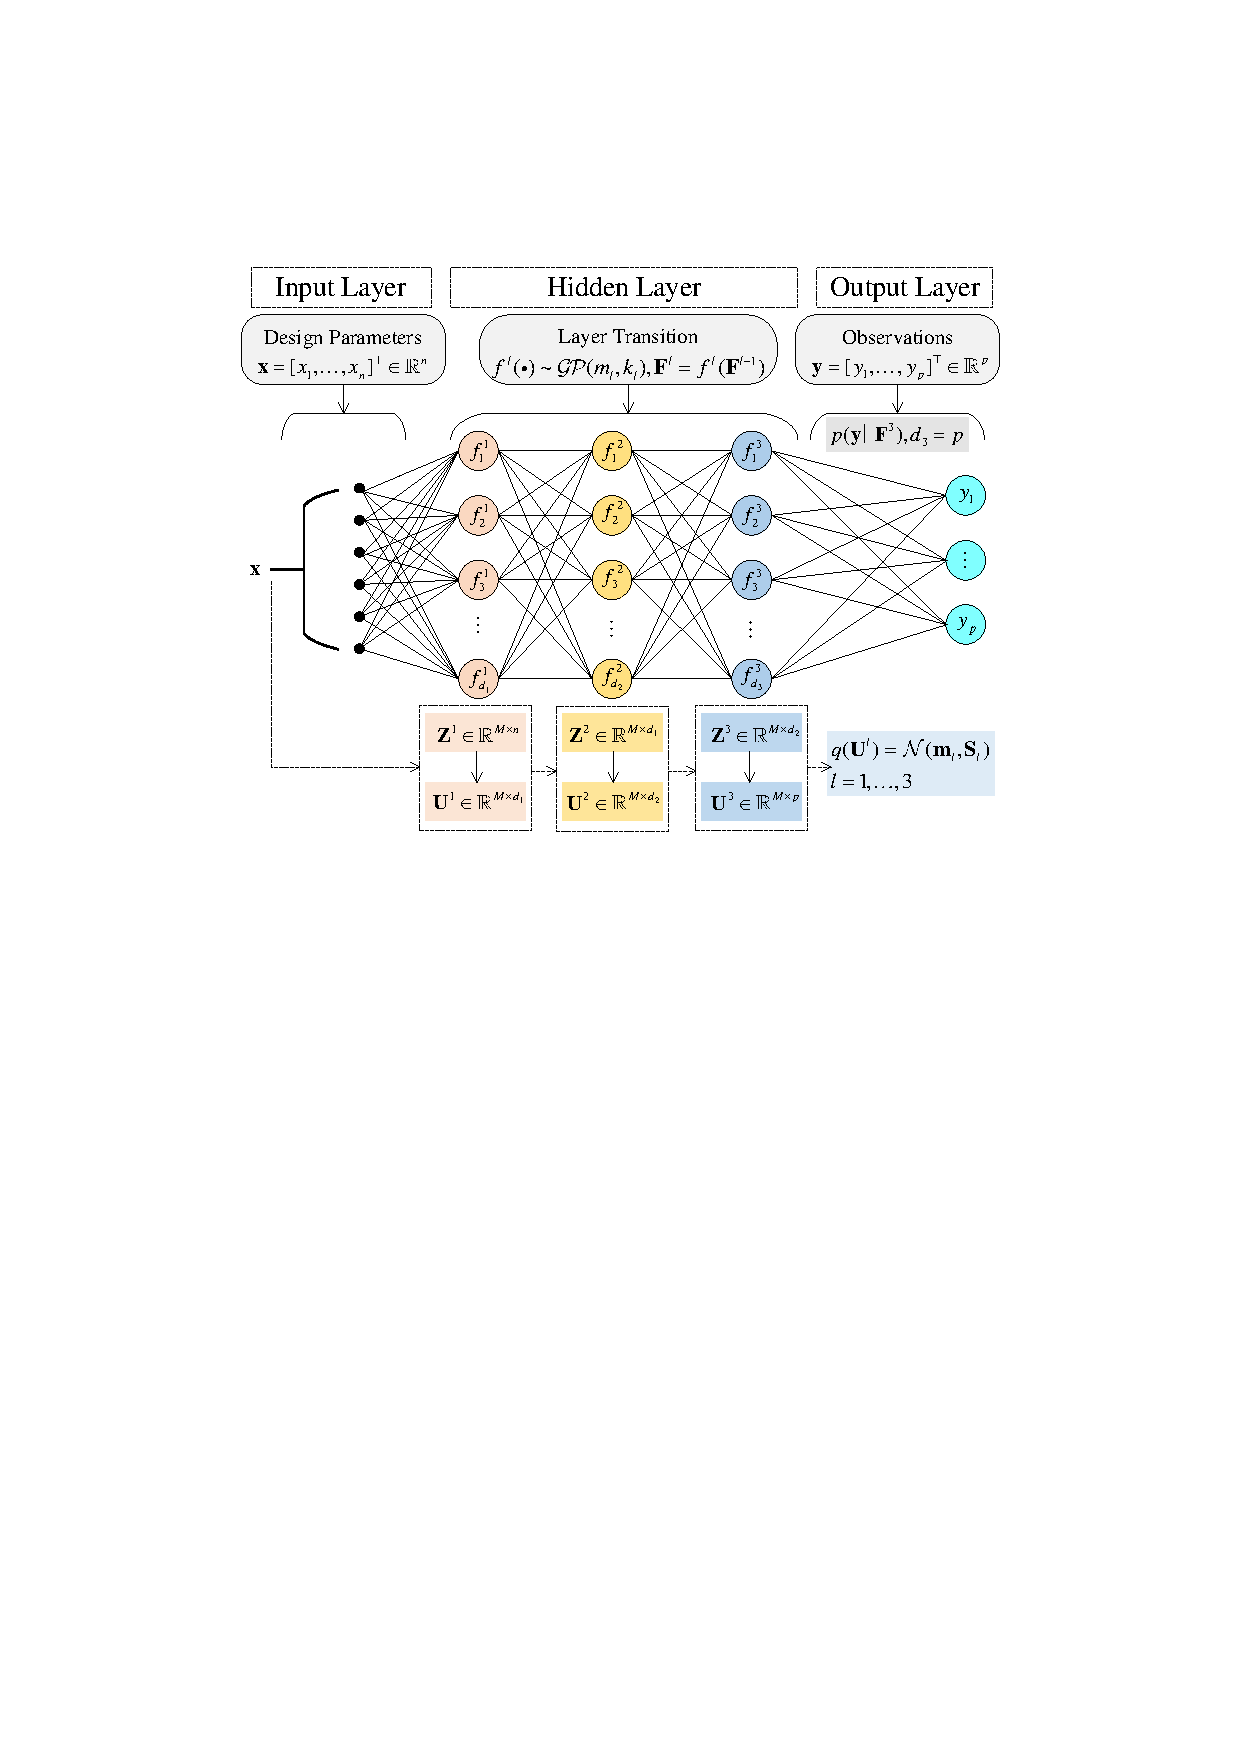
\includegraphics[width=0.9\linewidth]{FIG1.pdf}
	\caption{Architecture of the multi-output DGP. Connections represent probabilistic conditional dependencies rather than deterministic weights.}
	\label{fig:1}
\end{figure}

The generative process of an $L$-layer DGP is defined as a composition of functions $f^l(\cdot)$:
\begin{equation}
	{{\bf{F}}^0} = {\bf{X}}{\rm{ }},
\end{equation}
\begin{equation}
	{{\mathbf{F}}^{l}}\sim\mathcal{G}\mathcal{P}({{m}_{l}}({{\mathbf{F}}^{l-1}}),{{k}_{l}}({{\mathbf{F}}^{l-1}},{{\mathbf{F}}^{l-1}})),\quad l=1,\ldots ,L,
\end{equation}
where $\mathbf{F}^l$ denotes the matrix of function values at the $l$-th layer. The output layer of the model contains $p$ independent GP nodes, corresponding to the $p$ quality responses to be optimized. The observed data matrix $\mathbf{Y}$ is generated via the likelihood function $p(\mathbf{Y}|\mathbf{F}^L)$. To ensure computational feasibility, the concept of Sparse GPs (SGPs) is introduced at each layer, defining a set of inducing points $\mathbf{Z}^l$ and corresponding inducing variables $\mathbf{U}^l$. Consequently, the joint probability distribution of the DGP can be expressed as:
\begin{equation}
	p({\bf{Y}},\{ {{\bf{F}}^l},{{\bf{U}}^l}\} _{l = 1}^L) = p({\bf{Y}}|{{\bf{F}}^L})\prod\limits_{l = 1}^L p ({{\bf{F}}^l}|{{\bf{U}}^l},{{\bf{F}}^{l - 1}},{{\bf{Z}}^{l - 1}})p({{\bf{U}}^l};{{\bf{Z}}^{l - 1}}).
\end{equation}

Unlike the Linear Model of Coregionalization (LMC), this deep architecture implicitly captures nonlinear task correlations via shared latent representations. Since exact inference is intractable, variational inference is utilized. A layer-wise factorized variational posterior is specified to maintain the Markov property:
\begin{equation}
	q(\{ {{\bf{F}}^l},{{\bf{U}}^l}\} _{l = 1}^L) = \prod\limits_{l = 1}^L p ({{\bf{F}}^l}|{{\bf{U}}^l},{{\bf{F}}^{l - 1}},{{\bf{Z}}^{l - 1}})q({{\bf{U}}^l}){\rm{ }},
\end{equation}
where $q(\mathbf{U}^l)$ is the variational distribution of the inducing variables at the $l$-th layer. Based on this variational posterior, the ELBO for the multi-output DGP can be derived as:
\begin{equation}
	{{\mathcal{L}}_{\text{DGP}}}=\sum\limits_{k=1}^{p}{\sum\limits_{i=1}^{N}{{{\mathbb{E}}_{q(f_{i,k}^{L})}}}}[\log p({{y}_{i,k}}|f_{i,k}^{L})]-\sum\limits_{l=1}^{L}{\text{KL}}[q({{\mathbf{U}}^{l}})||p({{\mathbf{U}}^{l}};{{\mathbf{Z}}^{l-1}})].
\end{equation}

The expectation term in Equation (9) is analytically intractable due to the complex distributions induced by multiple nonlinear stochastic layers. Consequently, the Doubly Stochastic Variational Inference (DSVI) strategy \cite{Salimbeni2017} is adopted. Monte Carlo sampling is performed via the reparameterization trick: letting $\hat{\mathbf{f}}_i^0 = \mathbf{x}_i$ denote the input, samples are recursively generated for $l=1, \dots, L$ by first sampling a standard Gaussian noise vector:
\begin{equation}
	\epsilon _{i}^{l}\sim\mathcal{N}(\mathbf{0},{{\mathbf{I}}_{{{d}_{l}}}}).
\end{equation}
Then, the function values are updated via a deterministic transformation:
\begin{equation}
	\widehat{\mathbf{f}}_{i}^{l}={{\mathbf{\mu }}_{l}}(\widehat{\mathbf{f}}_{i}^{l-1})+\epsilon _{i}^{l}\odot \sqrt{\text{va}{{\text{r}}_{l}}(\widehat{\mathbf{f}}_{i}^{l-1})},
\end{equation}
where $\odot$ denotes the Hadamard product. This transformation allows gradients to backpropagate through the stochastic sampling step (proof in Appendix B). Combined with data subsampling, this constructs an unbiased ELBO estimator, enabling efficient end-to-end training via Mini-batch SGD.
However, the standard ELBO (9) represents an ``equal-weighted summation'' of reconstruction errors, effectively minimizing the global average error. This strategy fails to account for the conflicting nature of RPD objectives and the heterogeneous importance of samples for locating the optimal solution. To prioritize the ROI and critical responses, a weighted variational objective is formulated by introducing weights to the data fitting term:
\begin{equation}
	{{\mathcal{L}}_{Weighted}}=\sum\limits_{k=1}^{p}{\sum\limits_{i=1}^{N}{{{{\tilde{w}}}_{i,k}}}}{{\mathbb{E}}_{q(\mathbf{f}_{i,k}^{L})}}[\log p({{y}_{i,k}}|\mathbf{f}_{i,k}^{L})]-\sum\limits_{l=1}^{L}{\text{KL}}(q({{\mathbf{U}}^{l}})||p({{\mathbf{U}}^{l}})),
\end{equation}
where $\tilde{w}_{i,k}$ represents the composite weight for the $i$-th sample in the $k$-th task (generated by the dual-attention mechanism described later). This objective function can be interpreted as a criterion for ``preference-weighted" risk minimization, aiming to guide the model to allocate more learning capacity to the ROI and critical tasks. Obviously, when $\tilde{w}_{i,k}=1$, this objective degenerates to the standard ELBO.


\section{DA-DGP Modeling and Optimization} \label{s:sec3}
To synergize local refinement with global task balancing, a dual-layer multi-attention framework is proposed. This architecture hierarchically integrates static target-oriented sample attention to prioritize the ROI and dynamic meta-learning-driven task weighting to resolve objective conflicts. Through this design, microscopic exploitation and macroscopic coordination are unified to efficiently approximate the Pareto frontier.

\subsection{Target-Oriented Sample-Level Attention} \label{s:sec3.1}
The standard ELBO (Eq. 9) employs an equal-weight summation strategy, which inevitably dilutes fitting signals from the ROI critical for RPD. To mitigate this, a soft sample-level attention mechanism is introduced as a differentiable feature filter. By reconstructing the likelihood term, this mechanism compels the model to prioritize data subsets proximal to potential optimal solutions, thereby enhancing local prediction accuracy.

Specifically, consider a multi-task learning problem with $p$ response variables, where $y_{k}^{*}$ denotes the ideal target value predefined for the $k$-th task ($k \in \{1, \ldots, p\}$). Given the training dataset $\mathcal{D}=\{(\mathbf{x}_{i}, \mathbf{y}_{i})\}_{i=1}^{N}$ with observation vectors $\mathbf{y}_{i}=[y_{i,1}, \ldots, y_{i,p}]^{T}$, we quantify the relevance of sample $i$ to task $k$ using a Gaussian Radial Basis Function (RBF) kernel. This maps the Euclidean distance between the observation and the target to an attention score in $(0, 1]$. Consequently, the raw attention weight $s_{i,k}$ is defined as:
\begin{equation}
	{{s}_{i,k}}=\exp \left( -\frac{\|{{y}_{i,k}}-y_{k}^{*}{{\|}^{2}}}{2\sigma _{k}^{2}} \right),
\end{equation}
where $\|\cdot\|$ denotes the Euclidean norm and $\sigma_{k}$ controls the kernel bandwidth. This parameter modulates the attention decay rate: a smaller $\sigma_{k}$ induces a sharp focus on the immediate target vicinity, whereas a larger value expands the receptive field for broader coverage.

In practice, hyperparameters are specified based on domain knowledge rather than black-box optimization. The target $y_{k}^{*}$ is directly derived from design specifications (e.g., nominal values or theoretical bounds). The bandwidth $\sigma_{k}$ is determined via a data-driven heuristic, typically $\sigma_{k}=0.5 \cdot \text{std}(\mathbf{y}_{k})$, to ensure attention activation within the effective engineering range. To maintain numerical stability and scale consistency with the standard ELBO, the raw weights are normalized:
\begin{equation}
	{{\tilde{s}}_{i,k}}=\frac{{{s}_{i,k}}}{\sum\limits_{j=1}^{N}{{{s}_{j,k}}}}\cdot N  \qquad .
\end{equation}
This strategy ensures that $\sum_{i=1}^{N} \tilde{s}_{i,k} = N$. Based on these normalized weights, the expected log-likelihood term in Equation (9) is reconstructed. For task $k$, the sample-weighted loss function $\mathcal{L}'_{k}(\boldsymbol{\theta})$ can be expressed as:
\begin{equation}
	{{{\mathcal{L}}'}_{k}}(\boldsymbol{\theta })=\frac{1}{N}\sum\limits_{i=1}^{N}{{{{\tilde{s}}}_{i,k}}}\cdot {{\ell }_{k}}({{f}_{\boldsymbol{\theta }}}({{\mathbf{x}}_{i}}),{{y}_{i,k}}),
\end{equation}
where $\ell_{k}(\cdot)$ corresponds to the negative log-likelihood $-\log p(y_{i,k}|f_{i,k}^{L})$ in the first term of Equation (9). Integrating the normalized weights (15) into the standard variational framework (9) yields a preference-aware ELBO. The theoretical justification for this weighted objective, based on generalized variational inference, is provided in Appendix C. Consequently, the updated optimization objective $\mathcal{L}_{DGP}$ for $p$ tasks is formulated as:
\begin{equation}
	{{\mathcal{L}}_{DGP}}=\sum\limits_{k=1}^{p}{\left( \frac{1}{N}\sum\limits_{i=1}^{N}{{{{\tilde{s}}}_{i,k}}}\cdot \mathbb{E}\left[ \log p({{y}_{i,k}}|f_{i,k}^{L}) \right] \right)}-\sum\limits_{l=1}^{L}{\text{KL}}\left( q({{\mathbf{U}}^{l}})\|p({{\mathbf{U}}^{l}}) \right),
\end{equation}
where the first term utilizes normalized weights $\tilde{s}_{i,k}$ to bias the expected log-likelihood toward the Region of Interest (ROI), thereby dominating gradient updates; the second term imposes standard KL divergence regularization to prevent overfitting.

Statistically, Equation (16) implements a focused weighted likelihood estimation. The weights $\tilde{s}_{i,k}$ modulate the contribution of each observation to the posterior inference based on target proximity (Figure \ref{fig:2}). By amplifying update signals from critical regions while attenuating interference from irrelevant data fluctuations, this mechanism adaptively reallocates fitting resources to the ROI. Unlike hard-thresholding, this soft, differentiable filtering preserves information integrity and ensures gradient continuity, establishing a robust local foundation for subsequent multi-task balancing.

\begin{figure}[htbp]
	\centering
	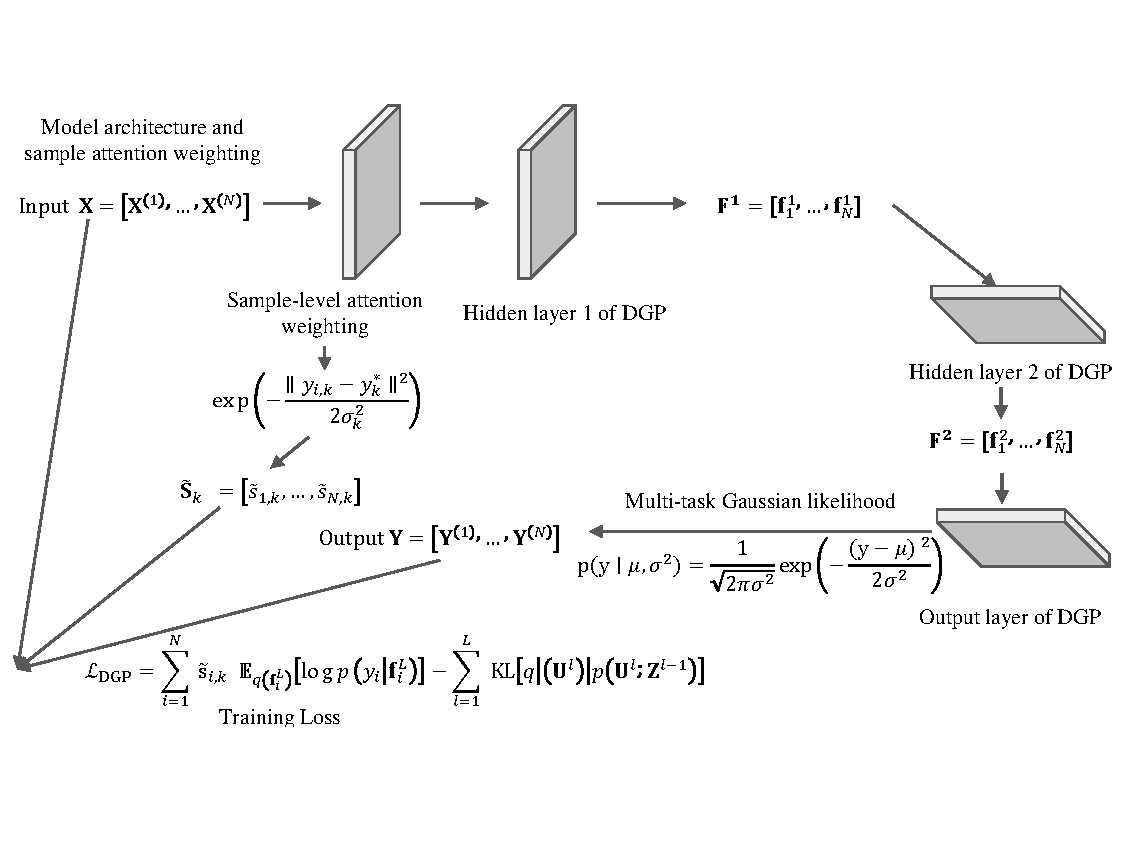
\includegraphics[width=0.7\linewidth]{FIG2.pdf}
	\caption{Schematic of the sample-level attention mechanism.}
	\label{fig:2}
\end{figure}

\subsection{Meta-Learning Driven Task-Level Dynamic Attention} \label{s:sec3.2}
While sample-level attention ensures microscopic local precision, the macroscopic challenge of conflicting objectives persists. In RPD, competing tasks often induce opposing gradient updates; consequently, static weighting strategies allow tasks with larger gradient magnitudes to dominate, impeding Pareto optimization. To resolve this, a meta-learning-driven dynamic task attention mechanism is introduced. Distinct from heuristic approaches like GradNorm \citep{Chen2018}, this method formulates a bilevel optimization problem. By leveraging feedback from an independent validation set, optimal task weights are learned adaptively to achieve end-to-end multi-task balancing.

\textbf{Construction of Bilevel Optimization Objective.} To achieve differentiable optimization of task weights, a learnable meta-parameter vector $\boldsymbol{\lambda} = [\lambda_1, \ldots, \lambda_p]^T \in \mathbb{R}^p$ is introduced. To satisfy the constraints that weights must be non-negative and sum to 1 (i.e., $\sum w_k = 1, w_k \ge 0$), the Softmax function is employed to map the meta-parameters to the final task attention weights $\mathbf{w}$:
\begin{equation}
	{{w}_{k}}(\boldsymbol{\lambda })=\frac{\exp ({{\lambda }_{k}})}{\sum\limits_{j=1}^{p}{\exp }({{\lambda }_{j}})},\quad k=1,\ldots ,p\text{ }.
\end{equation}
On this basis, the optimization process is formalized as a nested bilevel structure:

\textit{Inner Loop}: Responsible for updating the model parameters $\boldsymbol{\theta}$ of the DA-DGP (including variational parameters and inducing points). Its objective is to minimize the weighted loss function $\mathcal{L}_{\text{train}}$ on the training set. Here, the sample-weighted loss $\mathcal{L}'_k(\boldsymbol{\theta})$ derived in Equation (15) of Section 3.1 is directly invoked:
\begin{equation}
	{{\mathcal{L}}_{\text{train}}}(\boldsymbol{\theta },\boldsymbol{\lambda })=\sum\limits_{k=1}^{p}{{{w}_{k}}}(\boldsymbol{\lambda })\cdot {{{\mathcal{L}}'}_{k}}(\boldsymbol{\theta };{{\mathcal{D}}_{\text{train}}}).
\end{equation}

\textit{Outer Loop}: Responsible for updating the task weight meta-parameters $\boldsymbol{\lambda}$. Its objective is to maximize the generalization performance of the model on an independent validation set $\mathcal{D}_{\text{val}}$. The meta-objective function $\mathcal{L}_{\text{meta}}$ is defined as the weighted sum of task losses on the validation set:
\begin{equation}
	{{\mathcal{L}}_{\text{meta}}}({{\boldsymbol{\theta }}^{*}}(\boldsymbol{\lambda }))=\sum\limits_{k=1}^{p}{{{\pi }_{k}}}\cdot {{{\mathcal{L}}'}_{k}}({{\boldsymbol{\theta }}^{*}}(\boldsymbol{\lambda });{{\mathcal{D}}_{\text{val}}}),
\end{equation}
where $\pi_k$ ($\sum \pi_k = 1$) encodes the static engineering preference on the validation set, typically defaulting to $1/p$ for unbiased fitting. A critical distinction exists between $\pi_k$ and the dynamic training weights $\boldsymbol{\lambda}$: while $\boldsymbol{\lambda}$ adaptively modulates the optimization trajectory, $\pi_k$ defines the target equilibrium on the Pareto frontier. With $\boldsymbol{\theta}^*(\boldsymbol{\lambda}) = \arg \min_{\boldsymbol{\theta}} \mathcal{L}_{\text{train}}(\boldsymbol{\theta}, \boldsymbol{\lambda})$ representing the inner-loop solution, the global bilevel optimization objective is formulated as:
\begin{equation}
	\begin{aligned}
		& \min_{\boldsymbol{\lambda}} \mathcal{L}_{\text{meta}}(\boldsymbol{\theta}^*(\boldsymbol{\lambda})) \\
		& \text{s.t.} \quad \boldsymbol{\theta}^*(\boldsymbol{\lambda}) = \arg \min_{\boldsymbol{\theta}} \mathcal{L}_{\text{train}}(\boldsymbol{\theta}, \boldsymbol{\lambda})
	\end{aligned}.
\end{equation}

\textbf{Solution Strategy Based on One-step Gradient Look-ahead.} Given the computational intractability of deriving the exact inner optimum $\boldsymbol{\theta}^*(\boldsymbol{\lambda})$, a one-step gradient look-ahead approximation is employed. At training step $t$, a virtual parameter update is computed using the current weights $\boldsymbol{\lambda}$:
\begin{equation}
	\boldsymbol{{\theta }'}(\boldsymbol{\lambda })=\boldsymbol{\theta }-\alpha {{\nabla }_{\boldsymbol{\theta }}}{{\mathcal{L}}_{\text{train}}}(\boldsymbol{\theta },\boldsymbol{\lambda }).
\end{equation}
where $\alpha$ denotes the inner-loop learning rate. At this point, the difficulty of solving Equation (20) transforms into computing the gradient of the meta-objective function with respect to weights $\boldsymbol{\lambda}$. According to the chain rule, this gradient depends on the sensitivity of the updated virtual parameters $\boldsymbol{\theta}'$ to $\boldsymbol{\lambda}$:
\begin{equation}
	{{\nabla }_{\boldsymbol{\lambda }}}{{\mathcal{L}}_{\text{meta}}}={{\nabla }_{{\boldsymbol{{\theta }'}}}}{{\mathcal{L}}_{\text{meta}}}\cdot \frac{\partial \boldsymbol{{\theta }'}}{\partial \boldsymbol{\lambda }}.
\end{equation}

Noting that $\boldsymbol{\theta}'$ implicitly depends on $\boldsymbol{\lambda}$. Differentiating both sides of Equation (21) with respect to $\boldsymbol{\lambda}$ (treating $\boldsymbol{\theta}$ as a constant from the previous step), the Jacobian matrix is given by:
\begin{equation}
	\frac{\partial \boldsymbol{{\theta }'}}{\partial \boldsymbol{\lambda }}=-\alpha \nabla _{\boldsymbol{\theta },\boldsymbol{\lambda }}^{2}{{\mathcal{L}}_{\text{train}}}.
\end{equation}

Substituting Equation (23) back into Equation (22), the analytical expression for the meta-gradient is obtained:
\begin{equation}
	{{\nabla }_{\boldsymbol{\lambda }}}{{\mathcal{L}}_{\text{meta}}}\approx -\alpha {{\nabla }_{{\boldsymbol{{\theta }'}}}}{{\mathcal{L}}_{\text{meta}}}\cdot \nabla _{\boldsymbol{\theta },\boldsymbol{\lambda }}^{2}{{\mathcal{L}}_{\text{train}}}.
\end{equation}
Directly computing the Hessian matrix $\nabla_{\boldsymbol{\theta}, \boldsymbol{\lambda}}^2 \mathcal{L}_{\text{train}}$ is infeasible in high-dimensional parameter spaces. Therefore, this paper utilizes the finite difference method to efficiently approximate the Hessian-vector product. Given the direction vector $\mathbf{v} = \nabla_{\boldsymbol{\theta}'} \mathcal{L}_{\text{meta}}$, the second-order derivative term can be approximated as:
\begin{equation}
	\nabla _{\boldsymbol{\theta },\boldsymbol{\lambda }}^{2}{{\mathcal{L}}_{\text{train}}}\cdot \mathbf{v}\approx \frac{{{\nabla }_{\boldsymbol{\lambda }}}{{\mathcal{L}}_{\text{train}}}(\boldsymbol{\theta }+\epsilon \mathbf{v},\boldsymbol{\lambda })-{{\nabla }_{\boldsymbol{\lambda }}}{{\mathcal{L}}_{\text{train}}}(\boldsymbol{\theta }-\epsilon \mathbf{v},\boldsymbol{\lambda })}{2\epsilon }.
\end{equation}
Finally, the task weights $\boldsymbol{\lambda}$ are updated using this approximate gradient:
\begin{equation}
	\boldsymbol{\lambda }\leftarrow \boldsymbol{\lambda }-\beta {{\hat{\nabla }}_{\boldsymbol{\lambda }}}{{\mathcal{L}}_{\text{meta}}},
\end{equation}
where $\beta$ denotes the meta-learning rate, and $\hat{\nabla}_{\boldsymbol{\lambda}} \mathcal{L}_{\text{meta}}$ is the estimated gradient calculated by combining Equations (24) and (25).

\textbf{Algorithm Workflow.} The proposed method orchestrates a coupled dynamic optimization loop via alternating updates. In the inner loop, model parameters $\boldsymbol{\theta}$ are optimized against the weighted training loss to exploit local data features. Simultaneously, the outer loop leverages validation feedback to compute meta-gradients, dynamically rectifying task weights $\boldsymbol{\lambda}$ to prevent overfitting and autonomously navigate the Pareto frontier.

Despite the overhead of bilevel optimization, the computational cost remains feasible for RPD (typically $N<1000$), as it is dominated by the inherent complexity of GP inference. To ensure numerical stability, the implementation incorporates: (i) gradient clipping (threshold 1.0) to prevent explosion; (ii) decoupled learning rates ($\eta_{\theta} \gg \eta_{\lambda}$) to establish a stable ``fast-parameter, slow-weight'' dynamic; and (iii) Softmax activation to enforce weight non-negativity. The complete procedure is summarized in Algorithm \ref{alg:da_dgp}.

\begin{algorithm}[!h]
	\caption{DA-DGP modeling workflow.}
	\label{alg:da_dgp}
	\begin{spacing}{1}
%		\hrule
		\vspace{0.5\baselineskip}
	\begin{algorithmic}[1] % [1] 表示显示行号
		\Require Training set $\mathcal{D}_{\text{train}}$; Validation set $\mathcal{D}_{\text{val}}$; Number of tasks $p$; Target optimal values $\{y_{k}^{*}\}_{k=1}^{p}$; Gaussian kernel bandwidths $\{\sigma _{k}\}_{k=1}^{p}$; Validation preference weights $\{\pi _{k}\}_{k=1}^{p}$; Learning rates $\alpha, \beta$; Gradient clipping thresholds $\tau_{\text{in}}, \tau_{\text{out}}$; Finite difference perturbation step $\epsilon$; Maximum iterations $T$.
		\Ensure Trained model parameters $\boldsymbol{\theta}^*$; Final task weights $\mathbf{w}^*$.
		
		\State Initialize model parameters $\boldsymbol{\theta}$ and task attention meta-parameters $\boldsymbol{\lambda}$
		
		\State \textit{// Pre-computation of Sample-level Weights (Static)}
		\For{$k = 1$ to $p$}
		\State Compute raw weights: $s_{i,k} \gets \exp (-\|y_{i,k}-y_{k}^{*}\|^2 / 2\sigma_{k}^{2})$ for all $i=1 \dots N$
		\State Compute normalized weights: $\tilde{s}_{i,k} \gets (s_{i,k} / \sum_{j} s_{j,k}) \cdot N$
		\EndFor
		
		\State \textit{// Main Optimization Loop}
		\For{$t = 1$ to $T$}
		\State \textit{// Inner Loop: Virtual Update}
		\State Compute task weights: $\mathbf{w} \gets \text{softmax}(\boldsymbol{\lambda})$
		\State Compute weighted training loss: $\mathcal{L}_{\text{train}} \gets \sum_{k=1}^{p} w_{k} \cdot \mathcal{L}'_{k}(\boldsymbol{\theta})$ \Comment{Refer to Eq. (18)}
		\State Compute gradient and clip: $g_{\boldsymbol{\theta}} \gets \text{Clip}(\nabla_{\boldsymbol{\theta}} \mathcal{L}_{\text{train}}, \tau_{\text{in}})$
		\State Perform virtual parameter update: $\boldsymbol{\theta}' \gets \boldsymbol{\theta} - \alpha \cdot g_{\boldsymbol{\theta}}$
		
		\State \textit{// Outer Loop: Meta Update (Based on Validation Feedback)}
		\State Compute meta-loss on validation set: $\mathcal{L}_{\text{meta}} \gets \sum_{k=1}^{p} \pi_{k} \cdot \mathcal{L}'_{k}(\boldsymbol{\theta}'; \mathcal{D}_{\text{val}})$
		\State Compute gradient w.r.t virtual parameters: $\mathbf{v} \gets \nabla_{\boldsymbol{\theta}'} \mathcal{L}_{\text{meta}}$
		\State Approximate Hessian-vector product via Finite Difference: \Comment{Refer to Eq. (25)}
		\Statex \qquad $\mathbf{h} \approx \frac{\nabla_{\boldsymbol{\lambda}} \mathcal{L}_{\text{train}}(\boldsymbol{\theta} + \epsilon \mathbf{v}, \boldsymbol{\lambda}) - \nabla_{\boldsymbol{\lambda}} \mathcal{L}_{\text{train}}(\boldsymbol{\theta} - \epsilon \mathbf{v}, \boldsymbol{\lambda})}{2\epsilon}$
		\State Compute meta-gradient and clip: $g_{\boldsymbol{\lambda}} \gets \text{Clip}(-\alpha \cdot \mathbf{h}, \tau_{\text{out}})$
		\State Update meta-parameters: $\boldsymbol{\lambda} \gets \boldsymbol{\lambda} - \beta \cdot g_{\boldsymbol{\lambda}}$
		
		\State \textit{// Execute Real Parameter Update}
		\State $\boldsymbol{\theta} \gets \boldsymbol{\theta}'$
		\EndFor
		
		\State \Return $\boldsymbol{\theta}^* = \boldsymbol{\theta}$, $\mathbf{w}^* = \text{softmax}(\boldsymbol{\lambda})$
	\end{algorithmic}
\end{spacing}
%\hrule
\end{algorithm}

\subsection{Multi-Objective Robust Optimization Model} \label{s:sec3.3}
Following model training, the objective shifts to robust parameter optimization. To simultaneously minimize bias and variance, a multivariate expected quality loss is formulated based on Taguchi's quadratic loss framework \citep{Taguchi1986}. Leveraging the probabilistic posterior $y_{k}(\mathbf{x})\sim\mathcal{N}(\mu_{k}(\mathbf{x}),\sigma _{k}^{2}(\mathbf{x}))$ provided by DA-DGP, the classic loss function is generalized to the expected quality loss (EQL) for the $k$-th task \citep{Tan2012, Jiang2021}:
\begin{equation}
	E[{L_k}({\bf{x}})] = {C_k}\left[ {{{({\mu _k}({\bf{x}}) - y_k^*)}^2} + \sigma _k^2({\bf{x}})} \right].
\end{equation}

Equation (27) embodies robust design principles by simultaneously minimizing posterior mean deviation and variance. For multi-objective optimization, individual losses are aggregated into a global multivariate EQL metric using importance weights $\gamma_k$:
\begin{equation}
	J({\bf{x}}) = \sum\limits_{k = 1}^p {{\gamma _k}} E[{L_k}({\bf{x}})] = \sum\limits_{k = 1}^p {{\gamma _k}} {C_k}\left[ {{{({\mu _k}({\bf{x}}) - y_k^*)}^2} + \sigma _k^2({\bf{x}})} \right].
\end{equation}
Distinct from the dynamic training weights, $\gamma_{k}$ ($\sum\gamma_{k}=1$) represent static engineering priorities derived from cost or quality requirements. The RPD problem is thus cast as a constrained optimization within the design space $\Omega$:
\begin{equation}
	{{\bf{x}}^*} = \mathop {\arg \min }\limits_{{\bf{x}} \in \Omega } J({\bf{x}}).
\end{equation}
Given the non-convex nature of $J(\mathbf{x})$, a Genetic Algorithm (GA) is employed to identify the optimal process parameters $\mathbf{x}^{*}$ that minimize the global quality loss.

\section{Numerical and Engineering Validation} \label{s:sec4}
\subsection{Numerical Example} \label{s:sec4.1}
To evaluate the proposed method's efficacy in handling high-dimensional inputs and response heterogeneity, a synthetic benchmark with $\mathbf{x} \in [-1, 1]^5$ and three objectives is employed:
\begin{equation}
	\mathbf{y}(\mathbf{x})=\left[ \begin{matrix}
		{{y}_{1}}(\mathbf{x})  \\
		{{y}_{2}}(\mathbf{x})  \\
		{{y}_{3}}(\mathbf{x})  \\
	\end{matrix} \right]=\left[ \begin{matrix}
		\sin ({{x}_{1}})+0.5x_{2}^{2}-{{x}_{3}}+{{e}^{-{{x}_{4}}}}+\ln (1+x_{5}^{2})  \\
		{{x}_{1}}{{x}_{5}}+\cos ({{x}_{2}})+\sqrt{|{{x}_{3}}|+1}-\tanh ({{x}_{4}})  \\
		{{e}^{-0.5x_{1}^{2}}}+\ln (1+|{{x}_{2}}|)-{{x}_{3}}{{x}_{4}}+{{(|{{x}_{5}}|+0.1)}^{1/2}}  \\
	\end{matrix} \right].
\end{equation}
These responses represent escalating levels of complexity: $y_1$ serves as a smooth, separable baseline; $y_2$ introduces variable interactions and local non-differentiability; and $y_3$ exhibits significant non-convexity and complex coupling. This structural heterogeneity challenges standard fixed-weight optimization, thereby serving as a rigorous testbed for the proposed multi-attention mechanism. The optimization targets are set as $\mathbf{T}=[0, 1.5, 0.8]^T$.

\textbf{Evaluation Metrics and Baselines.} To comprehensively assess model performance, three metrics are employed: Root Mean Square Error (RMSE) to measure point prediction accuracy; Negative Log Predictive Density (NLPD) to evaluate the calibration quality of the probabilistic distributions; and Quality Loss (QL) to quantify the achievement of RPD goals by aggregating deviation and variance.
For comparative analysis, four representative baselines are selected: (i) EQUAL: The standard uniform weighting strategy \citep{Zhang2007}; (ii) UW: Uncertainty Weighting, which balances tasks via homoscedastic uncertainty \citep{Kendall2018}; (iii) DWA: Dynamic Weight Averaging, based on loss descent rates \citep{Liu2019}; and (iv) MGDA: Multi-Objective Gradient Descent, which seeks Pareto-descent directions \citep{Sener2018}. Additionally, two ablation variants are evaluated to isolate component contributions: T-Atten (retaining only task-level attention) and S-Atten (retaining only sample-level attention). Note that the latter is mathematically equivalent to the EQUAL baseline in this framework.

\textbf{Experimental Setup.} Latin Hypercube Sampling (LHS) is employed to generate $N=400$ training samples. Figure 3 validates the training stability and mechanism effectiveness by monitoring the convergence trajectories of three key components: the dynamic task weights (reflecting adaptive multi-task balancing), alongside the output scales $\sigma_f^2$ and ARD length-scales $l$ (confirming the capture of intrinsic data structures).

\begin{figure}[htb]
	\centering
	% 第一张子图 (a)
	\begin{subfigure}[b]{0.3\textwidth}
		\centering
		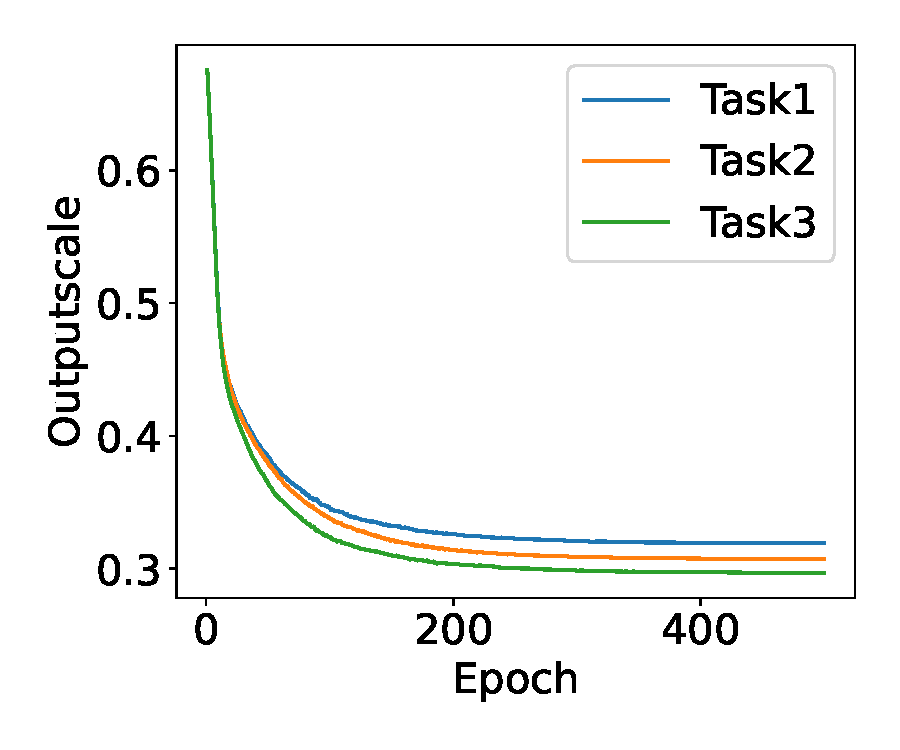
\includegraphics[width=\textwidth]{FIG3a.pdf}
		\caption{Variation of $\sigma_f^2$}
		\label{fig:sigma_variation}		
	\end{subfigure}
	\hfill % 弹性填充，让图片分布更均匀
	% 第二张子图 (b)
	\begin{subfigure}[b]{0.3\textwidth}
		\centering
		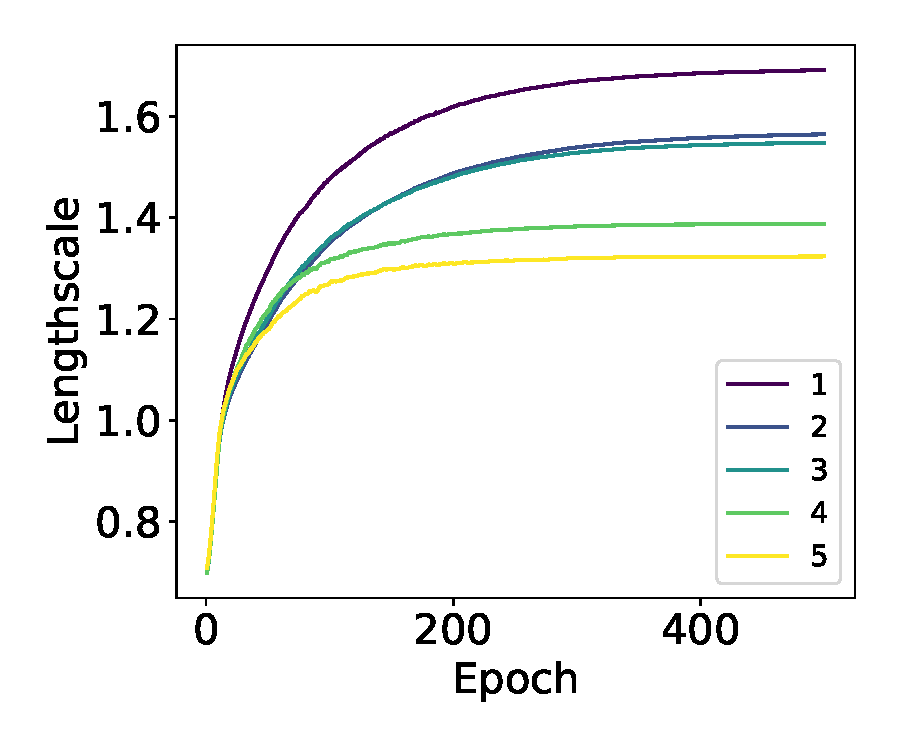
\includegraphics[width=\textwidth]{FIG3b.pdf}
		\caption{Variation of $l$}
		\label{fig:lengthscale_variation}
	\end{subfigure}
	\hfill
	% 第三张子图 (c)
	\begin{subfigure}[b]{0.3\textwidth}
		\centering
		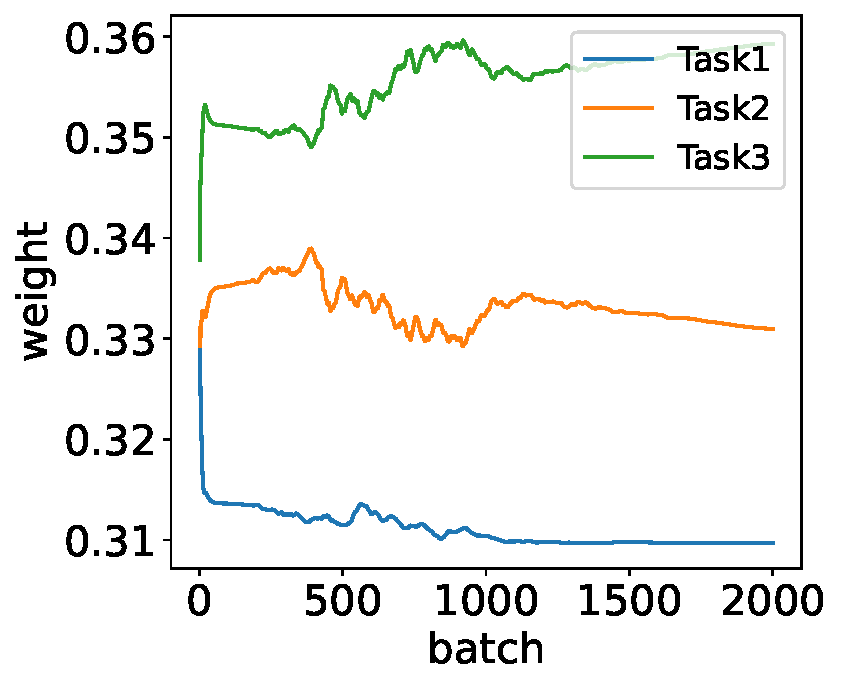
\includegraphics[width=\textwidth]{FIG3c.pdf}

		\caption{Variation of task weights}
		\label{fig:task_weights}
	\end{subfigure}
	
	\caption{Evolution trajectories of metrics during training.}
	\label{fig:evolution_metrics}
\end{figure}



Figures 3(a)-(b) depict the evolution of output scales ($\sigma_f^2$) and length-scales ($l$). The transition from initial fluctuations (exploration) to asymptotic convergence confirms the effective maximization of the log-marginal likelihood. Consequently, the stabilized parameters accurately characterize the inferred function smoothness and signal variance for each objective.
Figure 3(c) illustrates the dynamic weighting process. The rapid divergence in early training reflects the identification of task difficulty: weights for the complex Task 3 increase significantly, while those for the simple Task 1 decline. The resulting stable hierarchy (Task 3 > Task 2 > Task 1) mirrors the analytical complexity defined in Section 4.1. This confirms the mechanism's ability to adaptively reallocate resources and mitigate gradient dominance by simple tasks. Quantitative performance metrics (RMSE, NLPD, QL) averaged over 20 independent runs are detailed in Tables 1-3 (refer to Appendix D for visual comparisons).


\begin{table}[htbp]
	\centering
	\caption{Statistical results of metrics for Task 1 ($y_1$).}
	\label{tab:results_task1}
	\begin{tabular*}{\textwidth}{@{\extracolsep{\fill}}cccccccc}
		\toprule
		\textbf{Metric} & \textbf{Stat} & \textbf{DA-DGP} & \textbf{DWA} & \textbf{EQUAL} & \textbf{MGDA} & \textbf{UW} & \textbf{T-Atten} \\
		\midrule
		\multirow{6}{*}{RMSE} 
		& Max    & 0.0769 & 0.0756 & 0.1051 & 0.0786 & 0.0806 & 0.0687 \\
		& Min    & 0.0181 & 0.0185 & 0.0237 & 0.0170 & 0.0233 & 0.0170 \\
		& Median & 0.0311 & 0.0409 & 0.0443 & 0.0416 & 0.0488 & 0.0393 \\
		& Mean   & 0.0353 & 0.0422 & 0.0508 & 0.0436 & 0.0471 & 0.0404 \\
		& Q1     & 0.0246 & 0.0325 & 0.0343 & 0.0307 & 0.0338 & 0.0348 \\
		& Q3     & 0.0383 & 0.0486 & 0.0648 & 0.0541 & 0.0554 & 0.0433 \\
		\midrule
		\multirow{6}{*}{NLPD} 
		& Max    & -0.6971 & -0.4063 & -0.3736 & -0.4340 & -0.4108 & -0.7590 \\
		& Min    & -0.9025 & -0.5316 & -0.5211 & -0.6073 & -0.5165 & -0.8846 \\
		& Median & -0.8094 & -0.4742 & -0.4503 & -0.5071 & -0.4725 & -0.8226 \\
		& Mean   & -0.8097 & -0.4772 & -0.4550 & -0.5133 & -0.4720 & -0.8197 \\
		& Q1     & -0.8527 & -0.5112 & -0.4758 & -0.5537 & -0.4896 & -0.8440 \\
		& Q3     & -0.7757 & -0.4544 & -0.4408 & -0.4692 & -0.4556 & -0.7973 \\
		\midrule
		\multirow{6}{*}{QL}    
		& Max    & 0.0390 & 0.0706 & 0.0749 & 0.0669 & 0.0699 & 0.0349 \\
		& Min    & 0.0262 & 0.0550 & 0.0561 & 0.0472 & 0.0566 & 0.0271 \\
		& Median & 0.0315 & 0.0616 & 0.0646 & 0.0577 & 0.0617 & 0.0307 \\
		& Mean   & 0.0316 & 0.0614 & 0.0641 & 0.0573 & 0.0620 & 0.0309 \\
		& Q1     & 0.0289 & 0.0572 & 0.0614 & 0.0526 & 0.0598 & 0.0294 \\
		& Q3     & 0.0336 & 0.0641 & 0.0658 & 0.0623 & 0.0639 & 0.0321 \\
		\bottomrule
	\end{tabular*}
\end{table}

\begin{table}[htbp]
	\centering
	\caption{Statistical results of metrics for Task 2 ($y_2$).}
	\label{tab:results_task2}
	\begin{tabular*}{\textwidth}{@{\extracolsep{\fill}}cccccccc}
		\toprule
		\textbf{Metric} & \textbf{Stat} & \textbf{DA-DGP} & \textbf{DWA} & \textbf{EQUAL} & \textbf{MGDA} & \textbf{UW} & \textbf{T-Atten} \\
		\midrule
		\multirow{6}{*}{RMSE} 
		& Max    & 0.0541 & 0.0781 & 0.0723 & 0.0915 & 0.0686 & 0.0618 \\
		& Min    & 0.0215 & 0.0142 & 0.0233 & 0.0209 & 0.0223 & 0.0271 \\
		& Median & 0.0333 & 0.0404 & 0.0426 & 0.0416 & 0.0414 & 0.0390 \\
		& Mean   & 0.0358 & 0.0417 & 0.0448 & 0.0470 & 0.0437 & 0.0414 \\
		& Q1     & 0.0309 & 0.0338 & 0.0338 & 0.0358 & 0.0370 & 0.0323 \\
		& Q3     & 0.0415 & 0.0507 & 0.0543 & 0.0535 & 0.0518 & 0.0497 \\
		\midrule
		\multirow{6}{*}{NLPD} 
		& Max    & -0.6849 & -0.3897 & -0.3714 & -0.3936 & -0.4221 & -0.7430 \\
		& Min    & -0.8923 & -0.5612 & -0.5475 & -0.5965 & -0.5543 & -0.8812 \\
		& Median & -0.8097 & -0.4910 & -0.4744 & -0.4984 & -0.4791 & -0.8196 \\
		& Mean   & -0.8181 & -0.4894 & -0.4680 & -0.5006 & -0.4813 & -0.8189 \\
		& Q1     & -0.8638 & -0.5282 & -0.4922 & -0.5330 & -0.5013 & -0.8461 \\
		& Q3     & -0.7858 & -0.4547 & -0.4396 & -0.4785 & -0.4535 & -0.7928 \\
		\midrule
		\multirow{6}{*}{QL}    
		& Max    & 0.0404 & 0.0730 & 0.0756 & 0.0720 & 0.0684 & 0.0360 \\
		& Min    & 0.0267 & 0.0517 & 0.0532 & 0.0483 & 0.0525 & 0.0273 \\
		& Median & 0.0315 & 0.0596 & 0.0616 & 0.0586 & 0.0611 & 0.0308 \\
		& Mean   & 0.0312 & 0.0600 & 0.0626 & 0.0587 & 0.0609 & 0.0310 \\
		& Q1     & 0.0283 & 0.0553 & 0.0595 & 0.0547 & 0.0584 & 0.0293 \\
		& Q3     & 0.0330 & 0.0640 & 0.0660 & 0.0611 & 0.0643 & 0.0325 \\
		\bottomrule
	\end{tabular*}
\end{table}

\begin{table}[htbp]
	\centering
	\caption{Statistical results of metrics for Task 3 ($y_3$).}
	\label{tab:results_task3}
	\begin{tabular*}{\textwidth}{@{\extracolsep{\fill}}cccccccc}
		\toprule
		\textbf{Metric} & \textbf{Stat} & \textbf{DA-DGP} & \textbf{DWA} & \textbf{EQUAL} & \textbf{MGDA} & \textbf{UW} & \textbf{T-Atten} \\
		\midrule
		\multirow{6}{*}{RMSE} 
		& Max    & 0.2187 & 0.2317 & 0.2141 & 0.2372 & 0.2313 & 0.2065 \\
		& Min    & 0.0668 & 0.0837 & 0.0644 & 0.1062 & 0.0963 & 0.0878 \\
		& Median & 0.1158 & 0.1417 & 0.1394 & 0.1528 & 0.1369 & 0.1562 \\
		& Mean   & 0.1282 & 0.1448 & 0.1423 & 0.1584 & 0.1450 & 0.1517 \\
		& Q1     & 0.1072 & 0.1110 & 0.1162 & 0.1316 & 0.1247 & 0.1114 \\
		& Q3     & 0.1499 & 0.1670 & 0.1599 & 0.1815 & 0.1619 & 0.1850 \\
		\midrule
		\multirow{6}{*}{NLPD} 
		& Max    & -0.0603 & -0.0445 & -0.1034 & -0.0194 & -0.0432 & -0.1349 \\
		& Min    & -0.8055 & -0.4302 & -0.4300 & -0.4290 & -0.4248 & -0.7164 \\
		& Median & -0.5628 & -0.3421 & -0.3106 & -0.3040 & -0.3093 & -0.4198 \\
		& Mean   & -0.5289 & -0.2975 & -0.2951 & -0.2758 & -0.2989 & -0.4234 \\
		& Q1     & -0.6540 & -0.3641 & -0.3433 & -0.3353 & -0.3587 & -0.6364 \\
		& Q3     & -0.4457 & -0.2455 & -0.2616 & -0.2305 & -0.2775 & -0.2711 \\
		\midrule
		\multirow{6}{*}{QL}    
		& Max    & 0.0804 & 0.1078 & 0.1073 & 0.1135 & 0.1143 & 0.0771 \\
		& Min    & 0.0313 & 0.0668 & 0.0672 & 0.0662 & 0.0670 & 0.0368 \\
		& Median & 0.0477 & 0.0779 & 0.0816 & 0.0815 & 0.0813 & 0.0567 \\
		& Mean   & 0.0496 & 0.0824 & 0.0836 & 0.0846 & 0.0828 & 0.0559 \\
		& Q1     & 0.0411 & 0.0742 & 0.0781 & 0.0776 & 0.0756 & 0.0419 \\
		& Q3     & 0.0557 & 0.0924 & 0.0895 & 0.0888 & 0.0863 & 0.0665 \\
		\bottomrule
	\end{tabular*}
\end{table}



Based on the experimental data presented in Tables 1-3, the proposed DA-DGP demonstrates significant statistical advantages across three core metrics: RMSE, NLPD, and QL. Regarding prediction accuracy (RMSE), DA-DGP maintains the lowest average RMSE across all tasks, demonstrating its superior fitting capability. Specifically, in the high-complexity Task 3, compared to the DWA strategy, DA-DGP reduces the mean RMSE by approximately 11.5\% and the median by 18.2\%. This result strongly indicates that by assigning higher weights to difficult tasks via the task-level attention mechanism, the model successfully overcomes the common gradient dominance effect in multi-task learning, significantly enhancing the capture accuracy of non-stationary response surfaces. Notably, T-Atten outperforms EQUAL in simpler tasks (reducing Task 1 RMSE by 20.5\%), validating dynamic task balancing. However, its inferiority to DA-DGP in complex Task 3 (0.1517 vs. 0.1282) confirms sample-level attention is critical for capturing high-dimensional nonlinearities. Furthermore, DA-DGP achieves the smallest interquartile range (IQR) on Tasks 1 and 2, implying a more concentrated distribution of prediction errors and demonstrating strong robustness and stability across different training set partitions.

Regarding uncertainty quantification quality (NLPD), DA-DGP exhibits the most prominent advantage in this metric, which measures the quality of probabilistic predictions. Its average NLPD values for the three tasks improve to -0.81, -0.82, and -0.53, respectively (lower is better), significantly outperforming baselines such as MGDA and UW. This precision at the distributional level is attributed to the synergy between the deep structure of the multi-output DGP and the ARD mechanism. This enables the model not only to accurately predict the mean but also to output reasonable confidence intervals based on local data density, effectively avoiding the risks of overfitting or underfitting.

Regarding the achievement of robust design goals (QL), QL serves as the core metric for measuring the comprehensive performance of RPD. DA-DGP achieves the lowest mean and median QL across most tasks, with an IQR of only 0.0047 in Tasks 1 and 2, which is far lower than that of the comparative methods. This implies that the method is capable of minimizing both bias and variance simultaneously, achieving precise locking of the ROI. Even in the worst-case scenario (Max QL), DA-DGP maintains a lower loss upper bound, proving the focusing capability of the sample-level attention mechanism on critical regions under small sample conditions. This provides a highly reliable surrogate modeling foundation for subsequent parameter optimization.

In summary, the experimental results confirm the superiority of DA-DGP in handling high-dimensional heterogeneity. By synergizing local sample attention with global task weighting, the proposed mechanism optimizes the bias-variance trade-off, consistently outperforming baselines in RMSE, NLPD, and QL. These findings establish a robust algorithmic foundation for the subsequent case study: RPD of a 5G/6G OFDM communication system.


\subsection{Robust Parameter Design for OFDM Systems}\label{s:sec5.1}
To validate the proposed framework on complex engineering systems, this section presents a case study on the OFDM system, a core 5G/6G physical layer technology. System performance is constrained by strongly conflicting objectives: increasing transmission power improves SNR—enhancing Throughput and reducing BER—but inevitably degrades PAPR and energy consumption. Furthermore, the nonlinear coupling between multipath fading channels and Carrier Frequency Offset (CFO) induces highly non-stationary and heterogeneous response surfaces.

\begin{figure}[htbp]
	\centering
	\begin{subfigure}[b]{0.35\textwidth}
		\centering
		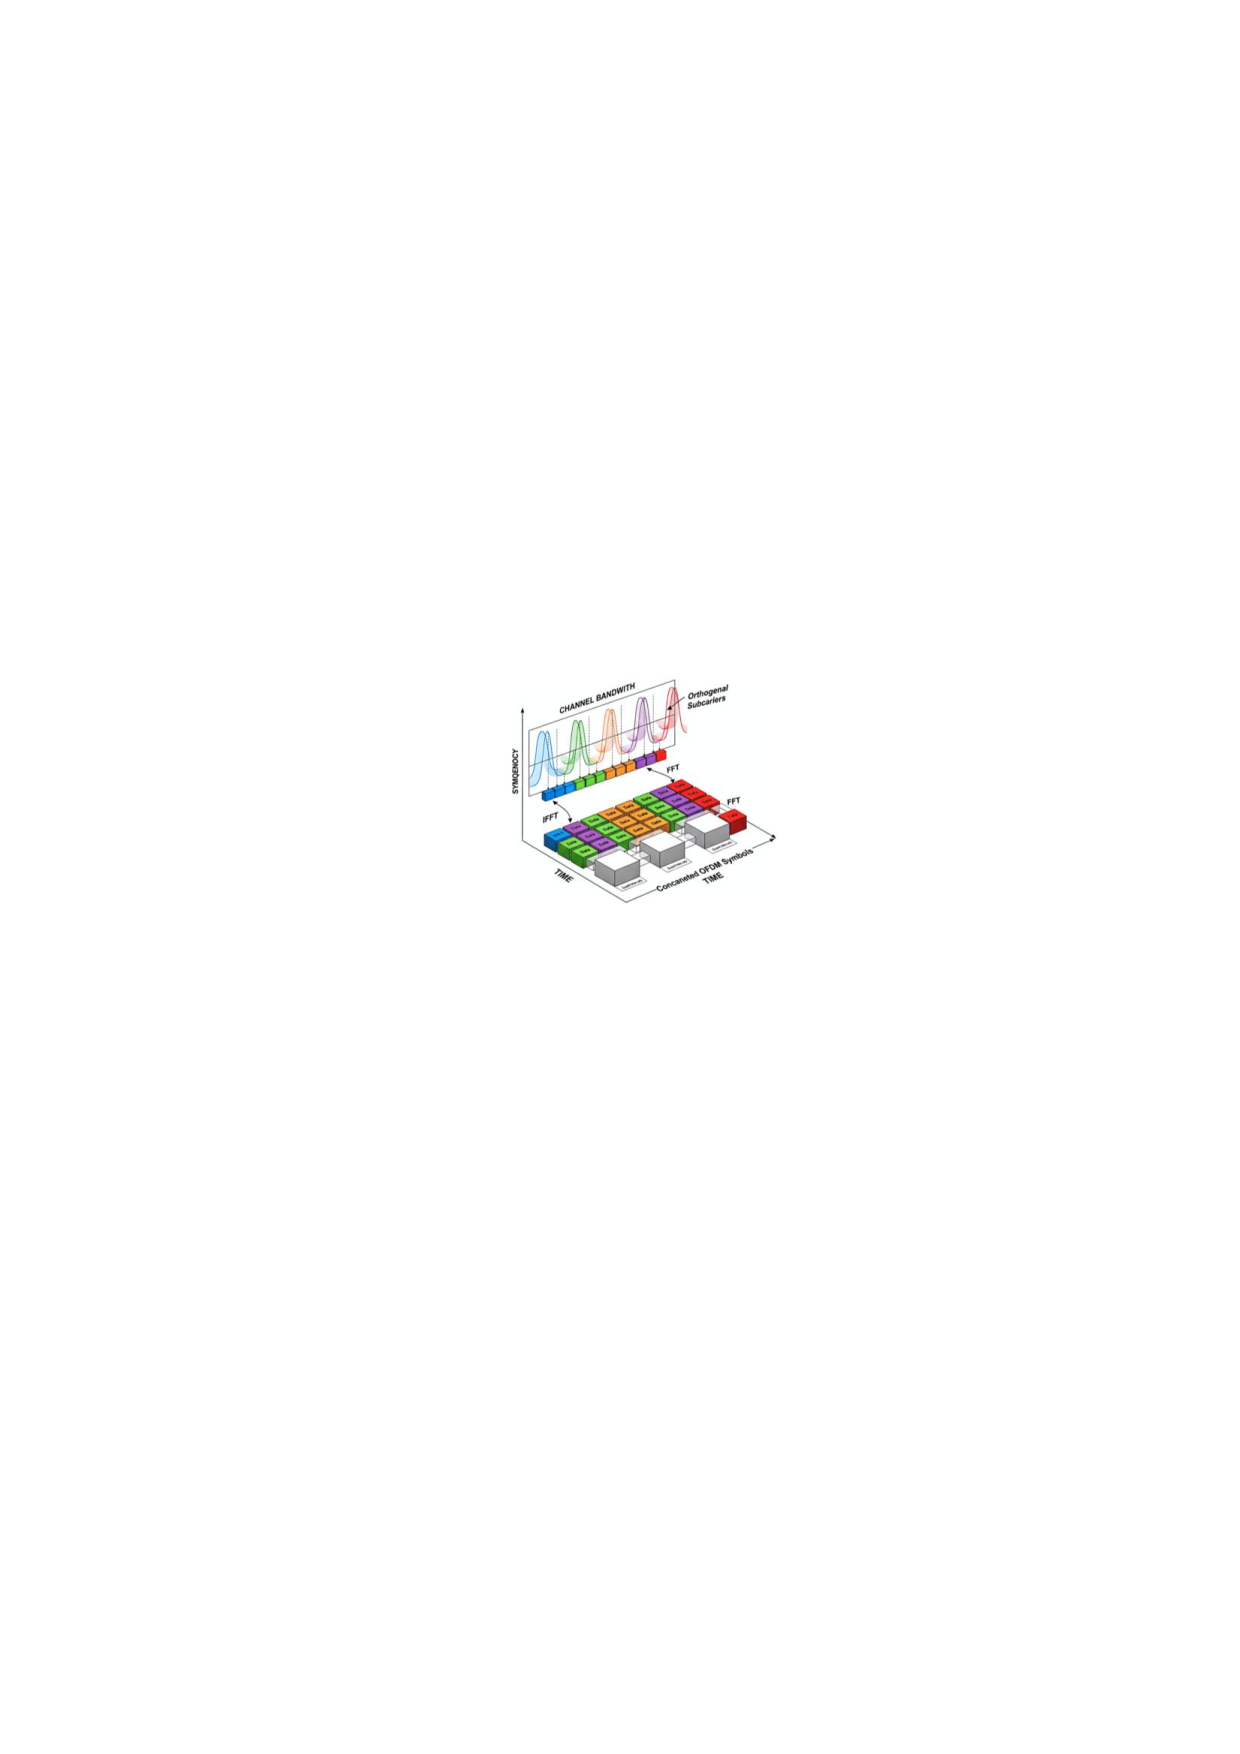
\includegraphics[width=\textwidth]{FIG5a.pdf} 
		\caption{OFDM signal structure}
		\label{fig:ofdm_signals}
	\end{subfigure}
%	\hfill 
	\begin{subfigure}[b]{0.35\textwidth}
		\centering
		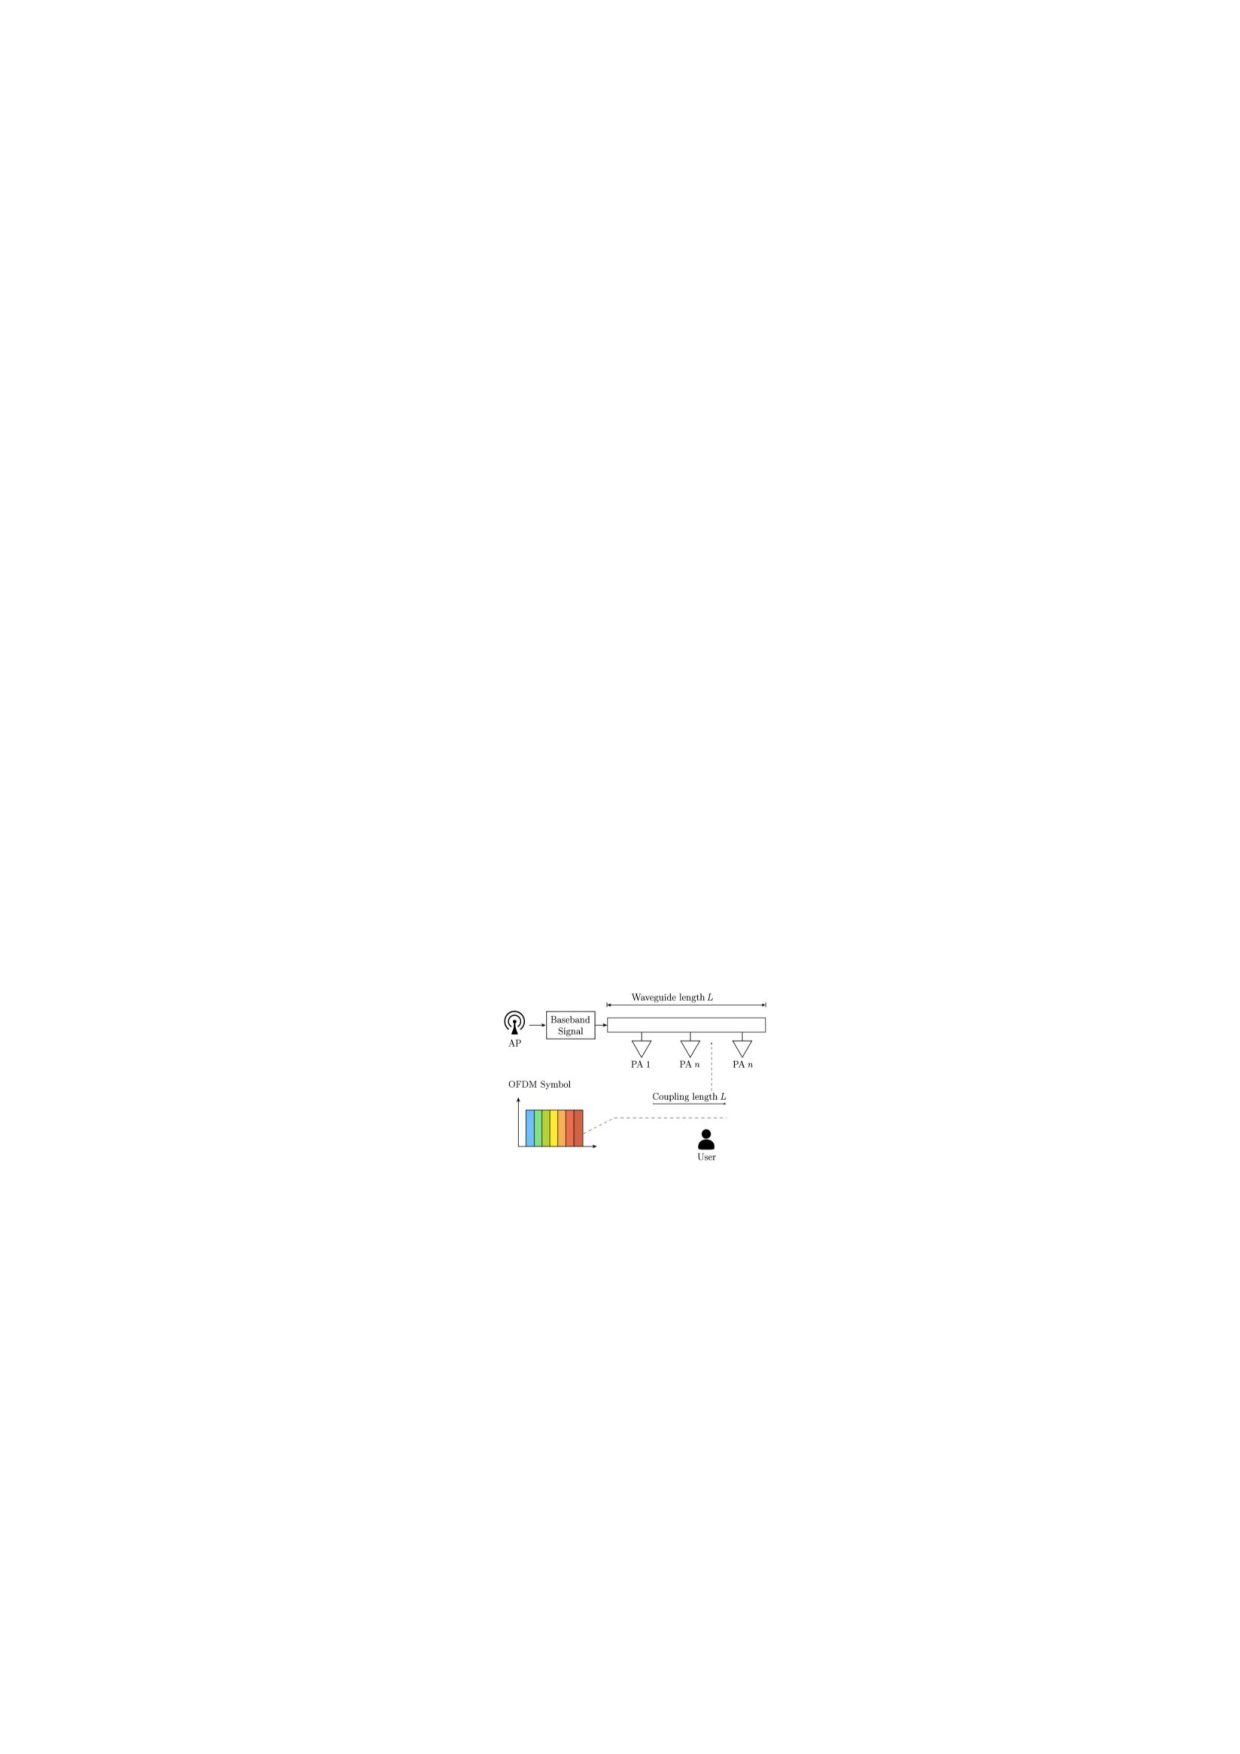
\includegraphics[width=\textwidth]{FIG5b.pdf}
		\caption{Pinching antenna system}
		\label{fig:pinching_system}
	\end{subfigure}

	\caption{Schematic diagrams of the proposed system.}
	\label{fig:combined_system}
\end{figure}

A high-fidelity OFDM simulation platform (Figure 4) is constructed operating at 3.5 GHz, employing 256-point FFT, 64-point CP, and 16-QAM. To characterize the impact of design factors $\mathbf{x}={{[{{x}_{1}},\ldots ,{{x}_{4}}]}^{T}}$ on responses $\mathbf{y}$, the simulation integrates three core physical mechanisms. First, the Energy Transmission Mechanism (${{x}_{1}},{{x}_{2}}$) determines SNR via transmit power ${{x}_{1}}$ and path loss distance ${{x}_{2}}$:
\begin{equation}
	SN{R_{dB}} = {x_1} - \left[ {20{{\log }{10}}\left( {\frac{{4\pi {f_c}}}{c}} \right) + 10{n{PL}}{{\log }{10}}\left( {\frac{{{x_2}}}{{{d_0}}}} \right)} \right] - {N{floor}},
\end{equation}
necessitating dynamic adjustment of ${{x}_{1}}$ to counteract ${{x}_{2}}$-induced nonlinear attenuation. Second, the Multipath Time Dispersion Mechanism (${{x}_{3}}$) models a Rayleigh fading channel with power delay profile (PDP) decay controlled by RMS delay spread ${{x}_{3}}$ ($PDP(\tau )\propto {{e}^{-\tau /{{x}_{3}}}}$); larger ${{x}_{3}}$ exacerbates frequency-selective fading and Inter-Symbol Interference (ISI), limiting BER. Third, the Spectral Offset Mechanism (${{x}_{4}}$) simulates Carrier Frequency Offset (CFO), introducing phase rotation ${{e}^{j2\pi \varepsilon k}}$ that destroys subcarrier orthogonality and generates Inter-Carrier Interference (ICI), degrading SINR. Collectively, these factors determine Throughput (${{y}_{1}}$), BER (${{y}_{2}}$), and PAPR (${{y}_{3}}$). Robustness is tested against challenging targets $\mathbf{T}={{[6.8\text{ Mbps}, 0.25, 10.6\text{ dB}]}^{T}}$ set at the feasible region boundaries.

In this experiment, Latin hypercube sampling (LHS) is employed to generate 400 initial samples within the design space $\Omega$ as the training set. The proposed DA-DGP model is then utilized to fit the complex nonlinear mapping $\mathbf{x} \to \mathbf{y}$. Based on the posterior mean $\mu_{i}(\mathbf{x})$ and variance $\sigma_{i}^{2}(\mathbf{x})$ predicted by the model, the expected quality loss (EQL) function for the $i$-th task is constructed as:
\begin{equation}
	{L_i}({\bf{x}}) = {({\mu _i}({\bf{x}}) - y_i^*)^2} + \sigma _i^2({\bf{x}}),\quad i = 1,2,3.
\end{equation}

Subsequently, the GA is adopted to solve the global optimization problem by minimizing the aggregated quality loss:
\begin{equation}
	\min_{\mathbf{x}\in\Omega} J(\mathbf{x}) = \sum_{i=1}^{3} L_i(\mathbf{x}).
	\label{eq:opt_objective}
\end{equation}
The optimal solution  $\mathbf{x}^*$ that minimize the composite metric $J(\mathbf{x})$ are selected as the final recommendation. To eliminate the impact of randomness, all optimization processes are run independently 20 times. The results are presented in Tables 4-5 and Figures 5-6.

\begin{table}[!h]
	\centering
	\caption{Summary of optimization results and validation comparisons.}
	\label{tab:sim_results}
	\begin{tabular*}{\textwidth}{@{\extracolsep{\fill}}cccccccc}
		\toprule
		\textbf{Metric} & \textbf{Stat} & \textbf{DA-DGP} & \textbf{DWA} & \textbf{EQUAL} & \textbf{MGDA} & \textbf{UW} & \textbf{T-Atten} \\
		\midrule
		\multirow{6}{*}{Throughput} 
		& Max    & 6.9198 & 6.8580 & 6.8609 & 6.6779 & 6.7336 & 6.4951 \\
		& Min    & 6.0717 & 5.8538 & 5.8189 & 6.1780 & 5.6536 & 6.2029 \\
		& Median & 6.5611 & 6.3679 & 6.2976 & 6.3573 & 6.1923 & 6.3486 \\
		& Mean   & 6.5427 & 6.3462 & 6.2682 & 6.3454 & 6.1970 & 6.3492 \\
		& Q1     & 6.4306 & 6.2221 & 6.0245 & 6.2624 & 6.0161 & 6.3163 \\
		& Q3     & 6.7909 & 6.5075 & 6.5359 & 6.4015 & 6.4438 & 6.3674 \\
		\midrule
		\multirow{6}{*}{BER} 
		& Max    & 0.2730 & 0.2991 & 0.3033 & 0.2603 & 0.3231 & 0.2573 \\
		& Min    & 0.1715 & 0.1789 & 0.1785 & 0.2004 & 0.1938 & 0.2223 \\
		& Median & 0.2144 & 0.2376 & 0.2460 & 0.2388 & 0.2586 & 0.2399 \\
		& Mean   & 0.2166 & 0.2402 & 0.2495 & 0.2403 & 0.2580 & 0.2398 \\
		& Q1     & 0.1869 & 0.2209 & 0.2175 & 0.2335 & 0.2285 & 0.2376 \\
		& Q3     & 0.2301 & 0.2550 & 0.2787 & 0.2502 & 0.2797 & 0.2437 \\
		\midrule
		\multirow{6}{*}{PAPR}    
		& Max    & 12.5554 & 12.6997 & 12.2940 & 12.7106 & 12.6997 & 13.0562 \\
		& Min    & 10.9274 & 10.8363 & 10.8322 & 11.1650 & 10.6603 & 11.6563 \\
		& Median & 11.5756 & 11.9866 & 11.5259 & 11.7655 & 11.6477 & 12.2653 \\
		& Mean   & 11.6618 & 11.9925 & 11.5305 & 11.7346 & 11.6868 & 12.3297 \\
		& Q1     & 11.2439 & 11.6781 & 11.1428 & 11.3945 & 11.1901 & 11.9886 \\
		& Q3     & 11.8033 & 12.5554 & 11.8646 & 12.1078 & 12.0574 & 12.4778 \\
		\bottomrule
	\end{tabular*}
\end{table}

\begin{table}[!h]
	\centering
	\caption{Statistical summary of QL for different methods.}
	\label{tab:quality_loss_results}
	\begin{tabular*}{\textwidth}{@{\extracolsep{\fill}}cccccccc}
		\toprule
		\textbf{Metric} & \textbf{Stat} & \textbf{DA-DGP} & \textbf{DWA} & \textbf{EQUAL} & \textbf{MGDA} & \textbf{UW} & \textbf{T-Atten} \\
		\midrule
		\multirow{6}{*}{Throughput} 
		& Max    & 0.3489 & 0.7932 & 0.8520 & 0.8545 & 0.9604 & 0.5909 \\
		& Min    & 0.1830 & 0.3834 & 0.4150 & 0.4626 & 0.4040 & 0.1858 \\
		& Median & 0.2461 & 0.5516 & 0.5857 & 0.7120 & 0.6196 & 0.2764 \\
		& Mean   & 0.2316 & 0.5363 & 0.5392 & 0.7273 & 0.5530 & 0.2580 \\
		& Q1     & 0.2035 & 0.4619 & 0.4969 & 0.6477 & 0.4977 & 0.2288 \\
		& Q3     & 0.2806 & 0.6168 & 0.6681 & 0.8063 & 0.7359 & 0.2922 \\
		\midrule
		\multirow{6}{*}{BER} 
		& Max    & 0.0096 & 0.0116 & 0.0112 & 0.0063 & 0.0068 & 0.0057 \\
		& Min    & 0.0027 & 0.0052 & 0.0057 & 0.0047 & 0.0054 & 0.0019 \\
		& Median & 0.0057 & 0.0070 & 0.0068 & 0.0051 & 0.0059 & 0.0036 \\
		& Mean   & 0.0052 & 0.0064 & 0.0064 & 0.0050 & 0.0059 & 0.0037 \\
		& Q1     & 0.0040 & 0.0058 & 0.0058 & 0.0048 & 0.0057 & 0.0026 \\
		& Q3     & 0.0074 & 0.0074 & 0.0074 & 0.0051 & 0.0062 & 0.0043 \\
		\midrule
		\multirow{6}{*}{PAPR}    
		& Max    & 0.8346 & 1.1072 & 0.9295 & 0.9669 & 0.9118 & 1.3655 \\
		& Min    & 0.3352 & 0.5290 & 0.5368 & 0.5254 & 0.4449 & 0.9686 \\
		& Median & 0.5740 & 0.7228 & 0.7512 & 0.6995 & 0.6754 & 1.1668 \\
		& Mean   & 0.5662 & 0.7001 & 0.8020 & 0.6752 & 0.6559 & 1.1666 \\
		& Q1     & 0.4874 & 0.6189 & 0.6657 & 0.6468 & 0.5725 & 1.0780 \\
		& Q3     & 0.6614 & 0.7675 & 0.8376 & 0.7581 & 0.7812 & 1.2518 \\
		\bottomrule
	\end{tabular*}
\end{table}

\begin{figure}[!h]
	\centering
	\begin{subfigure}[b]{0.32\textwidth}
		\centering
		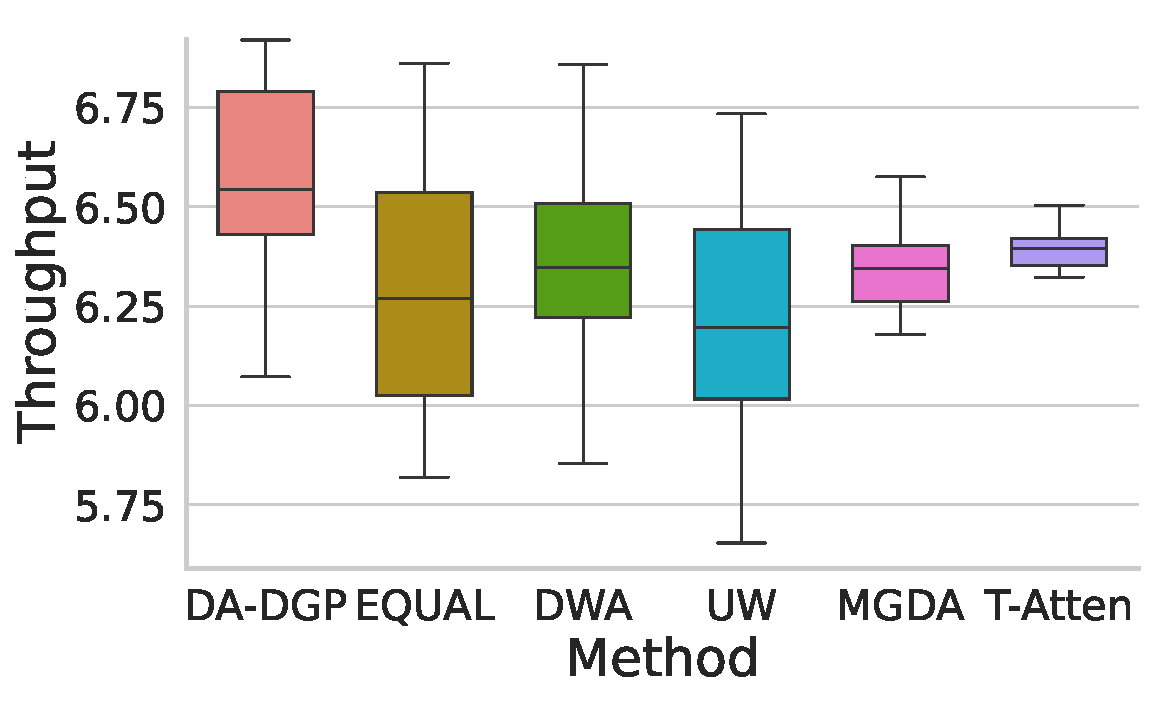
\includegraphics[width=\textwidth]{FIG6a.pdf} 
		\caption{Throughput}
		\label{fig:weights}
	\end{subfigure}
	\hfill 
	\begin{subfigure}[b]{0.32\textwidth}
		\centering
		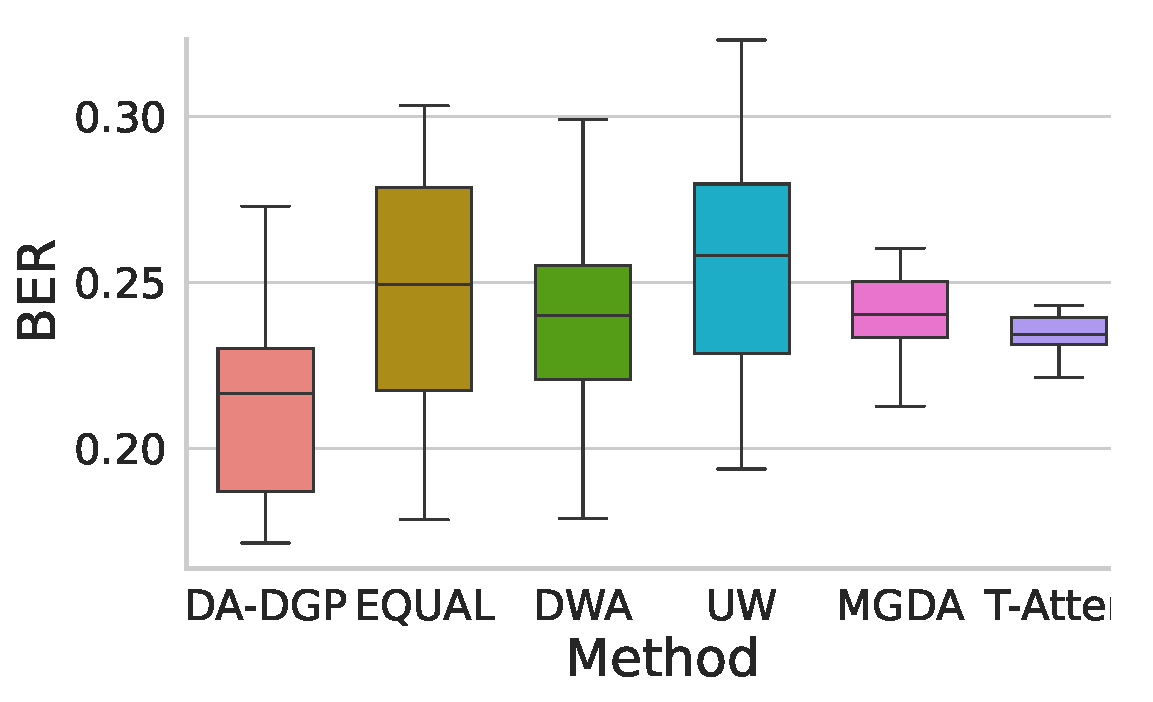
\includegraphics[width=\textwidth]{FIG6b.pdf}
		\caption{BER}
		\label{fig:sigma}
	\end{subfigure}
	\hfill
	\begin{subfigure}[b]{0.32\textwidth}
		\centering
		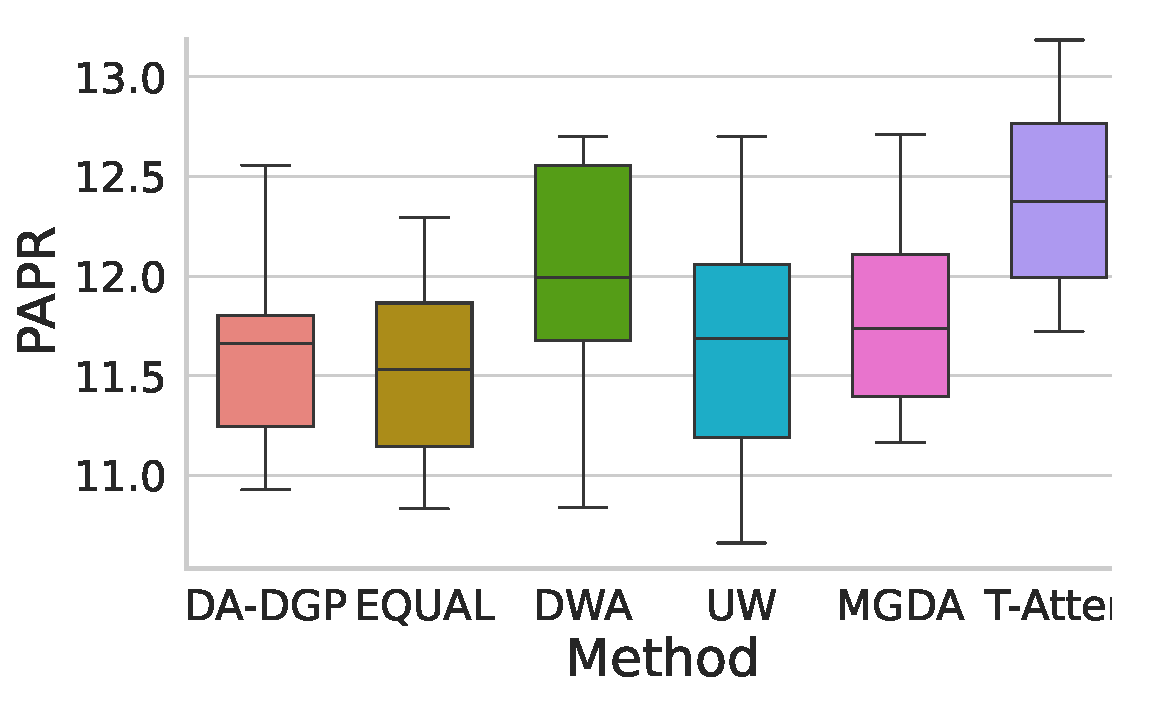
\includegraphics[width=\textwidth]{FIG6c.pdf}
		\caption{PAPR}
		\label{fig:lengthscale}
	\end{subfigure}
	\caption{Comparison of optimization results across different methods.}
	\label{fig:parameter_evolution}
\end{figure}


\begin{figure}[!h]
	\centering
	\begin{subfigure}[b]{0.32\textwidth}
		\centering
		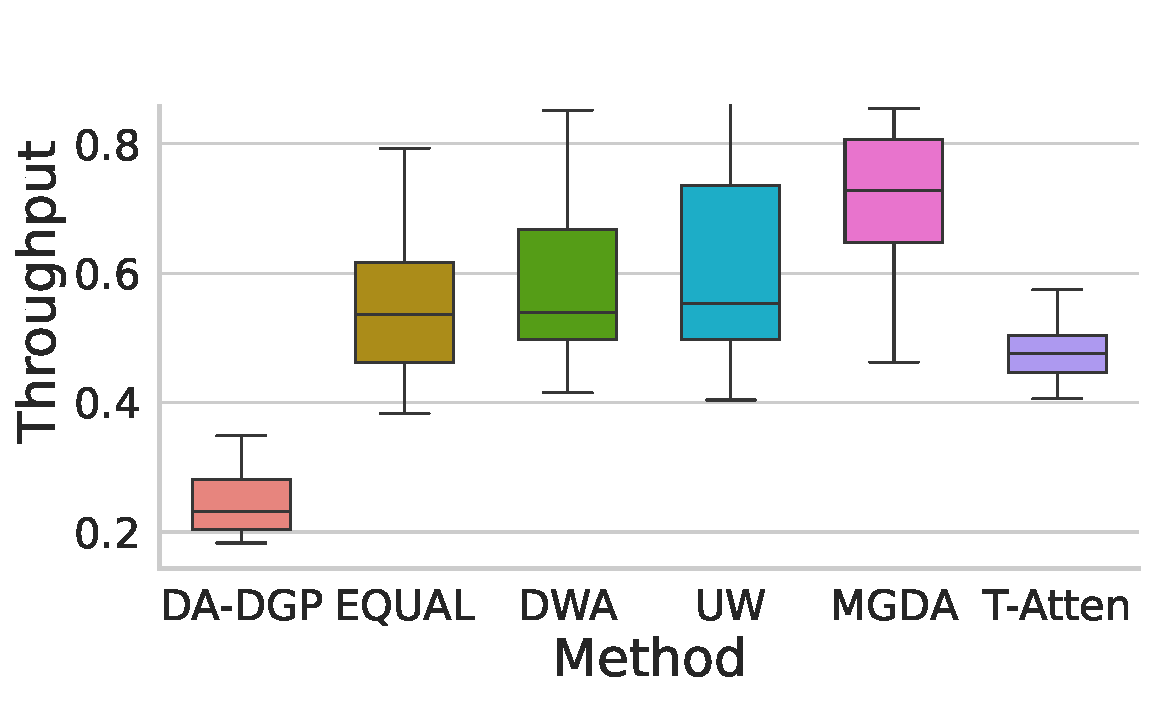
\includegraphics[width=\textwidth]{FIG7a.pdf} 
		\caption{Throughput}
		\label{fig:ql_throughput}
	\end{subfigure}
	\hfill
	\begin{subfigure}[b]{0.32\textwidth}
		\centering
		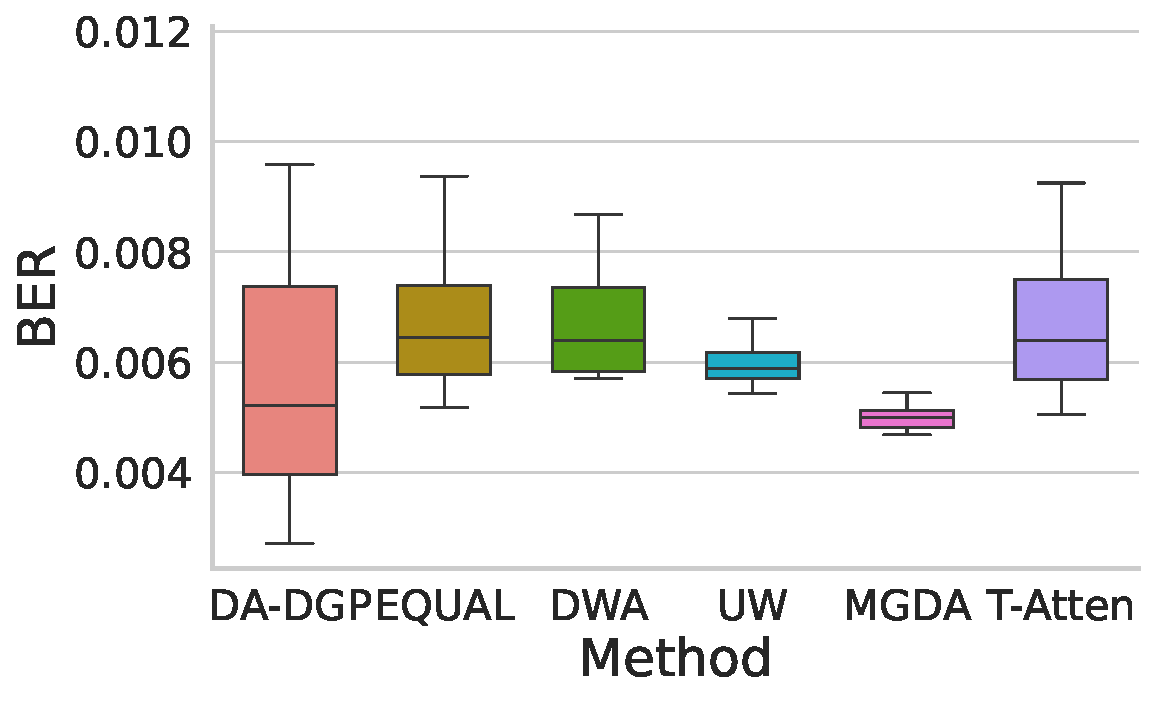
\includegraphics[width=\textwidth]{FIG7b.pdf}
		\caption{BER}
		\label{fig:ql_ber}
	\end{subfigure}
	\hfill
	\begin{subfigure}[b]{0.32\textwidth}
		\centering
		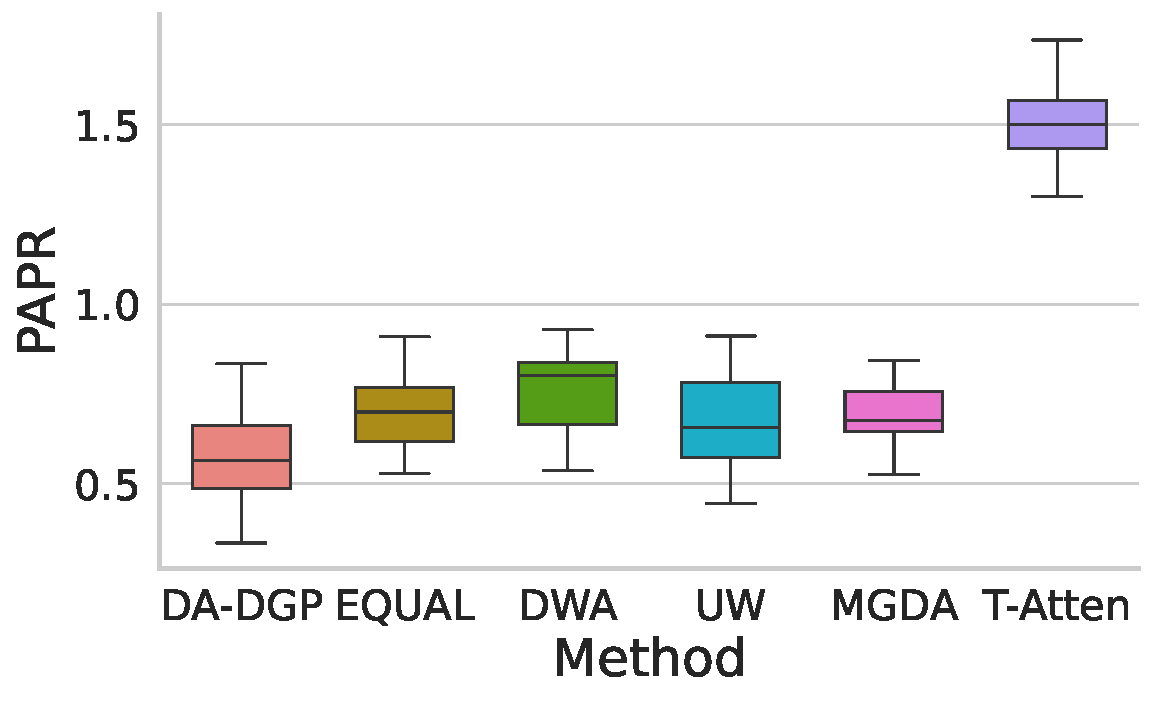
\includegraphics[width=\textwidth]{FIG7c.pdf}
		\caption{PAPR}
		\label{fig:ql_papr}
	\end{subfigure}
	\caption{Comparison of quality loss for optimization results across different methods.}
	\label{fig:quality_loss_comparison}
\end{figure}
\vspace{-0.5em}

Tables 4-5 and Figures 5-6 summarize the statistical performance and QL over 20 independent runs. The superiority of DA-DGP is demonstrated across three dimensions:

First, DA-DGP exhibits optimal trade-off capabilities in handling multi-objective conflicts. As shown in Figure 5, the method demonstrates significant distributional superiority: the boxplot for Throughput (maximization) shifts upwards with a median of 6.56 Mbps, significantly exceeding DWA and EQUAL. Conversely, boxplots for BER and PAPR (minimization) shift notably downwards. This confirms the dual-attention mechanism successfully guides the optimizer toward a superior Pareto frontier, avoiding suboptimal local extrema (e.g., MGDA's large positional deviation).

Second, Addressing the RPD goal of minimizing bias and variance, DA-DGP demonstrates engineering robustness in the comprehensive QL metric (Table 5 and Figure 6). For the QL of BER, DA-DGP achieves an IQR of only 0.0034 and a median of 0.0057—far lower than DWA (0.0070). This implies high consistency across runs and effective suppression of model uncertainty-induced ``performance drift".


Third, Controlling worst-case scenarios is critical in engineering practice. Table 4 shows DA-DGP significantly improves performance bounds: the minimum Throughput (6.07 Mbps) exceeds EQUAL (5.82 Mbps), and the maximum PAPR (12.56 dB) outperforms MGDA (12.70 dB). This demonstrates superior robustness against extreme channel conditions and parameter perturbations, effectively mitigating failure risks.

To visually validate effectiveness in a realistic environment, the optimal parameters $\mathbf{x}^{*}$ achieving the minimum composite quality loss were substituted into the high-fidelity OFDM simulation. Figures 7 and 8 evaluate the resulting signal modulation quality and system statistical characteristics, respectively.

\begin{figure}[!h]
	\centering
	% --- 第一行：3 张图 (DA-DGP, DWA, EQUAL) ---
	\begin{subfigure}[b]{0.28\textwidth}
		\centering
		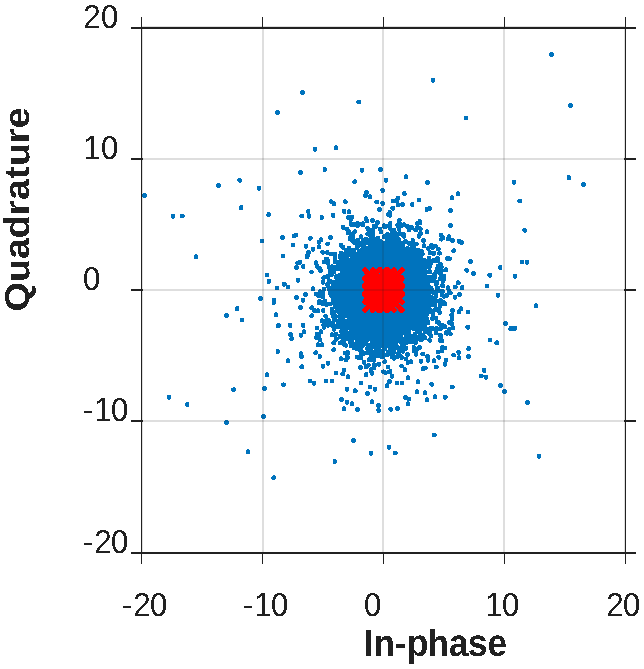
\includegraphics[width=\textwidth]{FIG8a.pdf}
		\caption{DA-DGP}
		\label{fig:const_pm}
	\end{subfigure}
	\hfill % 这里的 hfill 保证第一张和第二张之间的间距
	\begin{subfigure}[b]{0.28\textwidth}
		\centering
		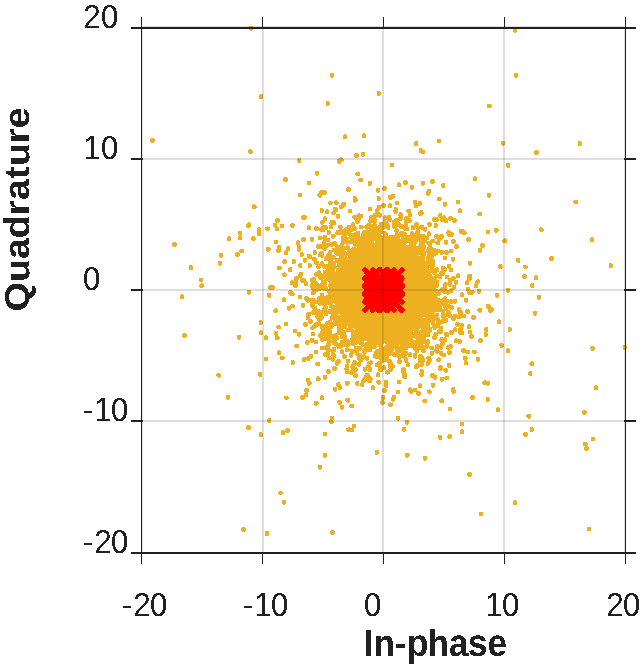
\includegraphics[width=\textwidth]{FIG8b.pdf}
		\caption{DWA}
		\label{fig:const_dwa}
	\end{subfigure}
	\hfill % 这里的 hfill 保证第二张和第三张之间的间距
	\begin{subfigure}[b]{0.28\textwidth}
		\centering
		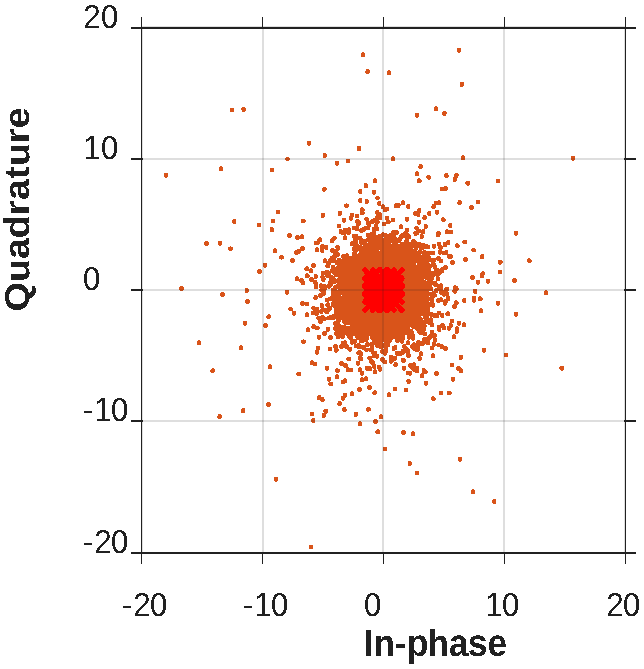
\includegraphics[width=\textwidth]{FIG8c.pdf}
		\caption{EQUAL} % 注意：您之前问过 S-Atten 是否等于 EQUAL，如果这里要对应消融实验，可以改为 "EQUAL (S-Atten)"
		\label{fig:const_equal}
	\end{subfigure}
	
	% --- 强制换行并增加垂直间距 ---
	\par\bigskip 
	% 或者使用 \vspace{1em} 来精确控制距离
	
	% --- 第二行：3 张图 (MGDA, UW, T-Atten) ---
	\begin{subfigure}[b]{0.28\textwidth}
		\centering
		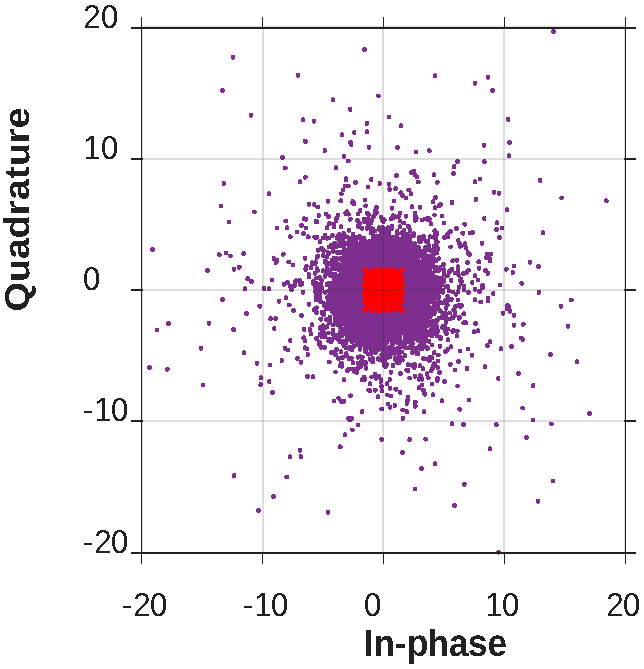
\includegraphics[width=\textwidth]{FIG8d.pdf}
		\caption{MGDA}
		\label{fig:const_mgda}
	\end{subfigure}
	\hfill % 弹性填充
	\begin{subfigure}[b]{0.28\textwidth}
		\centering
		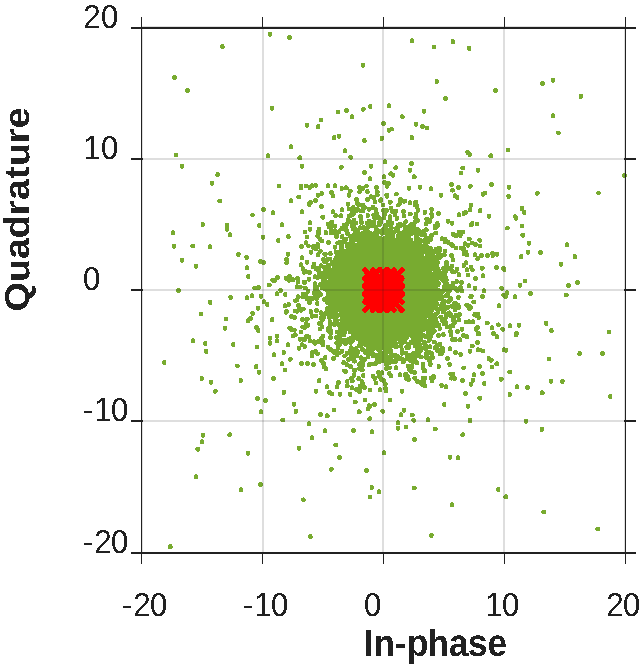
\includegraphics[width=\textwidth]{FIG8e.pdf}
		\caption{UW}
		\label{fig:const_uw}
	\end{subfigure}
	\hfill % 弹性填充
	\begin{subfigure}[b]{0.28\textwidth}
		\centering
		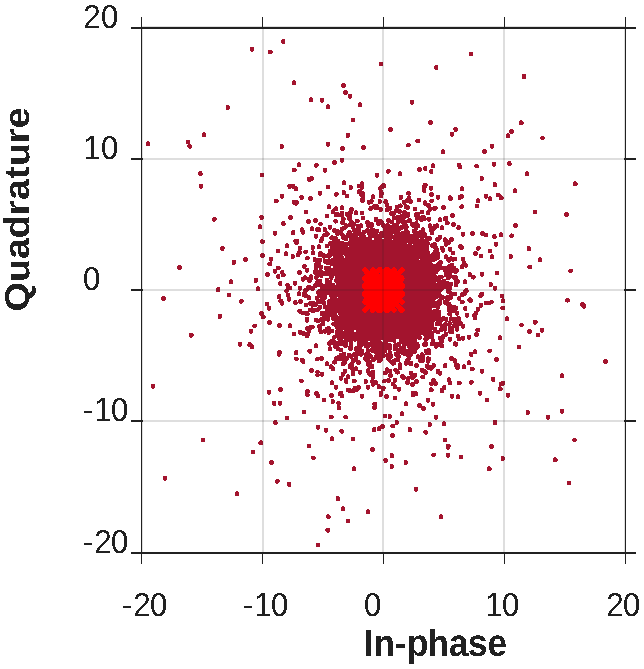
\includegraphics[width=\textwidth]{FIG8f.pdf}
		\caption{T-Atten}
		\label{fig:T-Atten}
	\end{subfigure}
	
	\caption{Constellation diagrams for each method.}
	\label{fig:constellation_diagrams}
\end{figure}



\begin{figure}[!h]
	\centering
	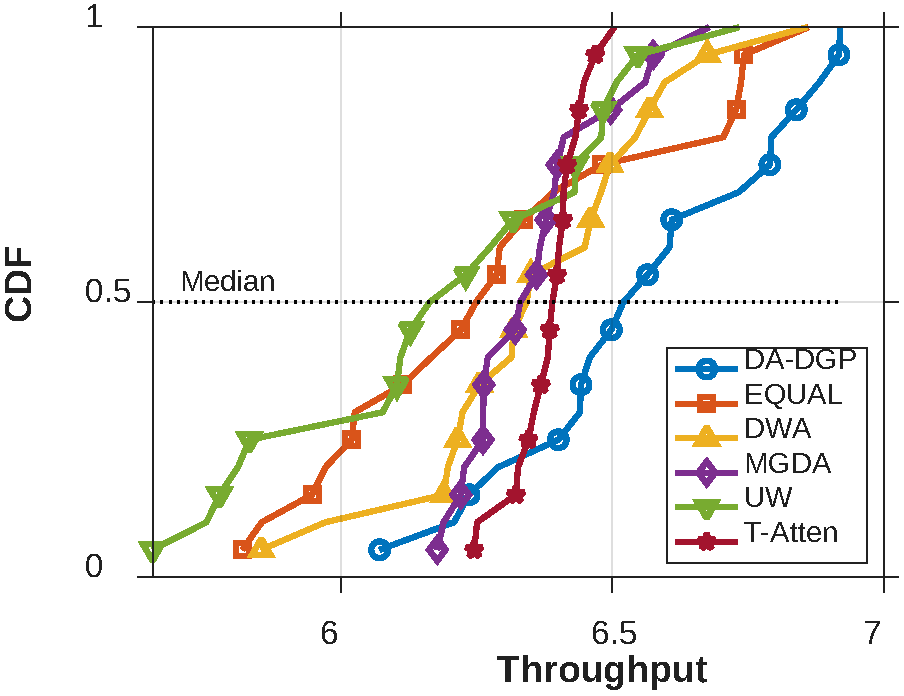
\includegraphics[width=0.4\textwidth]{FIG9.pdf}
	\caption{CDF of Throughput for different methods.}
	\label{fig:cdf_throughput}
\end{figure}


\begin{table}[!h]
	\centering
	\caption{Statistical summary of EVM.}
	\label{tab:evm_stats}
	\begin{tabular*}{\textwidth}{@{\extracolsep{\fill}}ccccccc}
		\toprule
		\textbf{Stat} & \textbf{DA-DGP} & \textbf{DWA} & \textbf{EQUAL} & \textbf{MGDA} & \textbf{UW} & \textbf{T-Atten} \\
		\midrule
		Max    & 13.3644 & 13.1080 & 23.3649 & 17.1535 & 14.2579 & 16.0728 \\
		Min    & 4.9181  & 3.8633  & 6.7667  & 5.3544  & 7.7372  & 5.3144 \\
		Mean   & 9.8258  & 10.1002 & 12.1678 & 10.4817 & 11.0535 & 9.9643 \\
		Median & 10.2415 & 10.1722 & 11.4234 & 10.1029 & 11.0828 & 9.9099 \\
		Q1     & 8.7413  & 9.2080  & 10.0786 & 8.8014  & 9.2834  & 8.2294 \\
		Q3     & 11.5257 & 12.2351 & 12.8316 & 11.6772 & 12.7877 & 11.4738 \\
		\bottomrule
	\end{tabular*}
\end{table}
\vspace{-0.5em}

Figure 7 displays the constellation diagram of the received signal on the complex plane, which serves as the ``gold standard" for measuring the physical layer quality of communication links. In contrast to the scattered and blurred states exhibited by baseline methods (Figs. 7b-e), the symbol points recovered by the DA-DGP method (Fig. 7a) form the most compact clusters around the ideal 16-QAM grid points. This visual result is corroborated by the EVM data in Table 6: the proposed method achieves the lowest mean EVM (9.83\%), representing a reduction of approximately 19.2\% compared to the EQUAL method (12.17\%). Crucially, the inferior worst-case performance of T-Atten (Max PAPR 13.06 dB vs. 12.56 dB for DA-DGP) indicates that task balancing alone cannot satisfy boundary constraints, necessitating sample-level attention for strict physical limitations. This confirms that the optimized parameter configuration (such as precise power allocation and pre-equalization strategies) effectively compensates for nonlinear channel distortions caused by multipath fading and carrier frequency offset.

Evaluation of cumulative distribution function CDF Throughput and system performance: The CDF curves in Figure 8 reveal the stability of the system's quality of service (QoS). The CDF curve of DA-DGP consistently yields higher throughput at the same cumulative probability compared to other methods, exhibiting distinct characteristics of first-order stochastic dominance. Statistically, a steeper CDF implies a smaller variance in the output distribution and more concentrated system performance. In contrast, although the MGDA method performs acceptably in the low-throughput region, it is significantly inferior in the high-throughput region (showing a distinct long-tail effect). Therefore, DA-DGP not only enhances average performance but also significantly strengthens the engineering reliability of the communication link across different channel states by compressing the long-tail distribution.

Combining the numerical case study with the OFDM engineering case, the proposed dual-attention DA-DGP framework demonstrates superior performance in addressing RPD problems characterized by small sample sizes, high-dimensional nonlinearities, and multi-objective conflicts. By compensating for channel impairments at the physical mechanism level and minimizing the bias and variance of quality loss at the statistical level, this method provides an efficient and robust technical path for intelligent resource scheduling and power control in 5G/6G communication systems.


\section{Conclusion}  \label{s:sec5}
A DA-DGP framework for the RPD of complex multi-output systems is proposed. The suggested algorithm takes advantage of an end-to-end weighted variational inference system, providing precise ROI focusing and adaptive task balancing by jointly optimizing dual-attention weights. The algorithm is shown empirically powerful in handling high-dimensional nonlinearities compared with benchmark methods, exhibited by the optimization of synthetic test functions. The proposed algorithm is applied to a high-fidelity 5G/6G OFDM simulation-based case study of optimizing communication link quality. Despite extremely small sample sizes, the algorithm was able to identify optimal parameters consistently for minimizing EVM. The inferior performances of the benchmark methods can be mainly attributed to the limitations of traditional ``mean-oriented" models and unmanaged gradient conflicts.

Empirical evaluations on numerical benchmarks and a 5G/6G OFDM system validate the superiority of the method. Statistically, DA-DGP consistently outperforms baselines (e.g., DWA, MGDA) in RMSE, NLPD, and QL metrics. In the engineering application, the optimized parameters yield the lowest Error Vector Magnitude (EVM) and steeper throughput convergence. These findings confirm the capability of the framework to mitigate long-tail performance risks and enhance link robustness, offering a promising path for intelligent parameter optimization in complex manufacturing and communication processes. 
A limitation of the current work lies in the reliance on the preset kernel bandwidth $\sigma_{k}$. Future research will focus on incorporating $\sigma_{k}$ directly into the variational inference framework. Realizing the adaptive learning of this hyperparameter based on data distribution characteristics will further improve the automation and generalizability of the model.




\if0\blind{
\section*{Data and Code Availability}
The code and data are available via the link https://zenodo.org/records/18263984.
%\vspace{-2em}
%\section*{Acknowledgements}
%This work was supported by the National Natural Science Foundation of China [Grant numbers 72301146, 72571142, 72561021, 72501133]; the China Postdoctoral Science Foundation (Grant number 2024T170430).	} \fi

\bibliographystyle{apalike}
%\bibliographystyle{Chicago}
\spacingset{1}
\bibliography{IISE-Trans}



	
\end{document}
